\documentclass[twocolumn,superscriptaddress,aps]{revtex4-1}

\usepackage[utf8]{inputenc}

\usepackage{amsfonts}
\usepackage{amssymb}
\usepackage{amsmath}
\usepackage{amsthm}

\usepackage{bbold}
\usepackage{bm}
\usepackage{graphicx}
\usepackage{color}
\usepackage{hyperref}
\usepackage{subcaption}
\usepackage{float}

\begin{document}


% ==============================================================================

\title{\Large{INFO8010: Interior Design Style Transfer}}
\vspace{1cm}
\author{\small{\bf Marie Goffin}}
\affiliation{\texttt{mgoffin@student.uliege.be} (\texttt{s191956})}
\author{\small{\bf Thomas Fredrich}}
\affiliation{\texttt{thomas.fredrich@student.uliege.be} (\texttt{s191717})}

\maketitle

% ==============================================================================

\section{Introduction}

Interior design visualization remains challenging for non-professionals. Most people struggle to imagine how their spaces would look in different design styles. Traditional visualization methods require either professional design skills or extensive photo editing expertise.\\

In this paper, we explore a machine learning approach for transforming room interior images between design styles. Our method investigates an enhanced CycleGAN architecture that aims to preserve structural elements while changing aesthetic features.\\

Our work examines:

\begin{itemize}
    \item Adapting CycleGAN for room style transfer
    \item Implementing multi-scale discriminators and improved residual blocks 
    \item Testing a structural preservation loss to maintain architectural elements
    \item Evaluating results using LPIPS and FID metrics
\end{itemize}

We focus specifically on transferring between industrial and scandinavian bathroom styles. Our approach works with unpaired datasets, addressing the practical limitation that paired before/after images of the same room in different styles are rarely available.

\section{Related Work}

\subsection{Image-to-Image Translation}
Image-to-image translation has seen significant progress in recent years. Pix2Pix \cite{isola2017image} introduced a general framework for supervised image translation using conditional GANs, requiring paired training data. CycleGAN \cite{zhu2017unpaired} extended this approach to the unpaired setting by introducing cycle consistency loss, enabling training without directly corresponding before/after images. This unpaired approach is particularly valuable for interior design applications, where obtaining before/after photos of the same room in different styles is difficult.

\subsection{Style Transfer}
Neural style transfer, explored by Gatys et al. \cite{gatys2016image}, showed the ability to transfer artistic styles to photographs using feature representations from pre-trained networks. Subsequent approaches improved efficiency \cite{johnson2016perceptual} and versatility \cite{huang2017arbitrary}. In particular, adaptive instance normalization (AdaIN) \cite{huang2017arbitrary} and whitening and coloring transforms (WCT) \cite{li2017universal} demonstrated better separation of content and style. While these methods work well for artistic style transfer, they often struggle with the structural preservation needs of interior design applications.

\subsection{Diffusion Models}
More recently, diffusion-based generative models have shown exceptional capabilities in image generation and manipulation tasks. Denoising diffusion probabilistic models (DDPM) \cite{ho2020denoising} introduced a new paradigm for high-quality image synthesis. These techniques have evolved into powerful text-to-image models such as DALL-E 2 \cite{ramesh2022hierarchical} and latent diffusion models \cite{rombach2022high}. 

While these models can produce impressive style transformations with text guidance, they typically require large-scale training data and computational resources. Some recent work has explored using diffusion models specifically for image-to-image translation tasks \cite{saharia2022palette}, though often with different training requirements compared to GAN-based approaches.

\subsection{Interior Design Applications}
Image translation and style transfer techniques have been applied to interior design in both academic research and commercial applications. Several existing tools offer interior visualization capabilities. Our work builds upon Fu \cite{fu2022digital}, who demonstrated promising results by enhancing CycleGAN for art style transfer. 

We adapt Fu's architectural modifications—including improved residual blocks, multi-scale discriminators, and specialized loss functions—specifically for room style transfer. While newer diffusion-based approaches show promise, we chose to work with CycleGAN for its established ability to work with unpaired image datasets of modest size and its more accessible computational requirements.

\section{Methodology}

\subsection{Dataset}

Our project uses a subset of bathroom interior images sourced from the "Interior Design Images and Metadata Dataset from Pinterest" (available on Kaggle as "galinakg/interior-design-images-and-metadata"). The original dataset contained multiple room types (bathroom, bedroom, kitchen, living room) with various design styles, accompanied by CSV metadata files linking images to style categories and attributes.

For our implementation, we made several modifications to the dataset:

\begin{itemize}
    \item We focused exclusively on bathroom images to enable our model to specialize in a single room type
    \item We cleaned the dataset to remove:
      \begin{itemize}
        \item Images containing text/writing
        \item Images showing only color palettes
        \item Images with single objects rather than complete rooms
      \end{itemize}
    \item We removed the CSV metadata files and instead organized images directly into style-specific directories
\end{itemize}

While the original dataset contained five bathroom design styles (boho, industrial, minimalist, modern, and scandinavian), we chose to work with \textbf{industrial} and \textbf{scandinavian} styles. This decision was based on the clear visual contrast between these styles—industrial bathrooms typically feature raw, utilitarian elements with exposed materials and metal fixtures, while scandinavian bathrooms are characterized by light, airy spaces with natural materials and neutral colors. We reasoned that this strong stylistic difference would make the style transfer effects more pronounced and easier to evaluate.\\

For training our model, we split each style category into train (70\%), validation (15\%), and test (15\%) sets. This resulted in approximately 105 industrial and 79 scandinavian bathroom images for training, with proportional numbers for validation and testing.

\subsection{Model Architecture}

Our architecture is based on CycleGAN \cite{zhu2017unpaired} with several enhancements inspired by Fu \cite{fu2022digital}. The overall system consists of two generator networks and two discriminator networks, enabling bidirectional translation between industrial and scandinavian bathroom styles. Figure~\ref{fig:architecture} illustrates the high-level architecture of our system.

\begin{figure}[htbp]
    \centering
    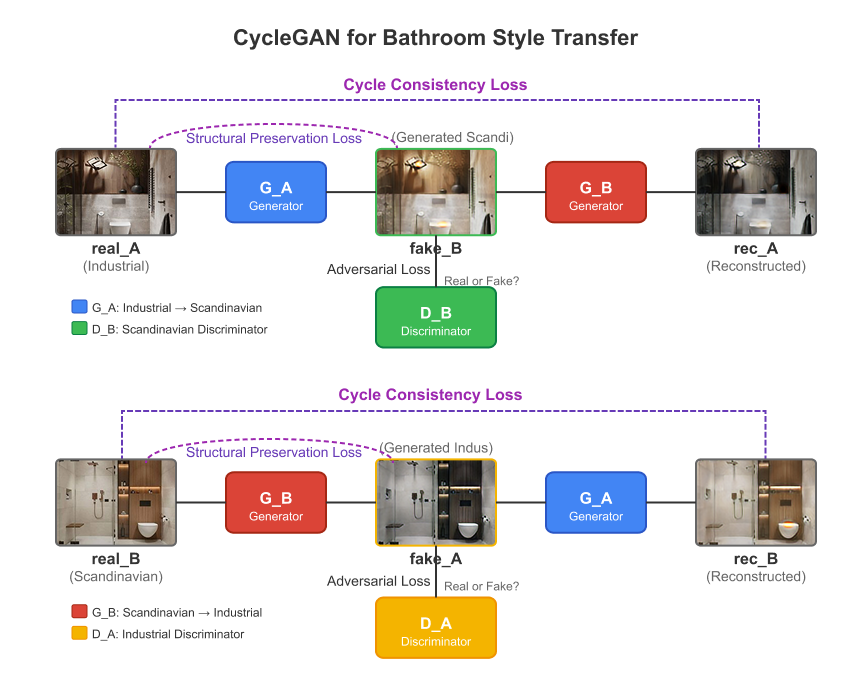
\includegraphics[width=0.5\textwidth]{assets/cyclegan_architecture.png}
    \caption{CycleGAN architecture for bathroom style transfer between Industrial and Scandinavian styles, showing generators (G$_A$, G$_B$), discriminators (D$_A$, D$_B$), and our integrated loss functions.}
    \label{fig:architecture}
\end{figure}

\subsubsection{Generator Architecture}

Our generator network uses a ResNet-based architecture tailored for interior design style transfer:

\begin{itemize}
    \item Initial reflection padding and 7×7 convolution to preserve edge information, which is critical for maintaining bathroom structural elements
    \item Two downsampling layers with stride-2 convolutions and instance normalization
    \item Nine residual blocks for feature transformation while maintaining spatial information
    \item Bilinear interpolation upsampling followed by 3×3 convolutions to reduce checkerboard artifacts (edge distortions caused by convolutional operations at image boundaries) common in transpose convolutions
    \item Final reflection padding and 7×7 convolution with Tanh activation
\end{itemize}

The dual generator structure allows us to create both Industrial→Scandinavian (G$_A$) and Scandinavian→Industrial (G$_B$) transformations. This bidirectionality enables cycle consistency training without requiring paired images.

\subsubsection{Multi-scale Discriminator}

To better capture both global structure and local details, we implemented a multi-scale discriminator that operates at two resolutions:

\begin{itemize}
    \item Full-resolution discriminator for capturing overall image coherence and stylistic patterns
    \item Half-resolution discriminator for focusing on larger-scale features (like layout and fixtures)
    \item Each discriminator uses a PatchGAN architecture with spectral \cite{miyato2018spectral} normalization for training stability
\end{itemize}

This multi-scale approach helps the model better distinguish between industrial and scandinavian styles while maintaining structural coherence. For example, the full-resolution discriminator might focus on detailed textures like tile patterns or fixture finishes, while the half-resolution discriminator captures more general properties like color schemes and spatial arrangements.

\subsubsection{Perceptual Network}

For our structural preservation loss, we incorporated a perceptual network based on pre-trained VGG19 features. This network extracts features at three different depths, allowing us to capture different levels of structural information:

\begin{itemize}
    \item Low-level features (edges, textures) from early layers, which help preserve basic elements like walls and fixtures
    \item Mid-level features (patterns, local structures) from middle layers, capturing bathroom fixtures and their arrangement
    \item High-level features (spatial arrangements) from deeper layers, representing overall bathroom layout
\end{itemize}

By weighting these feature levels differently in our loss function (with higher weight on low and mid-level features), we encourage the model to preserve structural elements while still allowing stylistic changes appropriate for the target domain. This is especially important for bathroom style transfer, where we want to maintain the layout and fixtures while changing decorative elements to match either industrial or scandinavian design aesthetics.

\subsection{Loss Functions}
Our training objective combines several loss terms:
\begin{equation}
\mathcal{L} = \mathcal{L}_{GAN} + \lambda_{cycle}\mathcal{L}_{cycle} + \lambda_{id}\mathcal{L}_{id} + \lambda_{struct}\mathcal{L}_{struct}
\end{equation}

\subsubsection{Adversarial Loss}
We use the GAN loss with mean squared error (MSE) for training stability:
\begin{equation}
\mathcal{L}_{GAN}(G, D) = \mathbb{E}_{y}[(D(y) - 1)^2] + \mathbb{E}_{x}[D(G(x))^2]
\end{equation}

\subsubsection{Cycle Consistency Loss}
This loss ensures that transformed images can be mapped back to their original versions:
\begin{equation}
\mathcal{L}_{cycle} = \mathbb{E}_{x}[||G_B(G_A(x)) - x||_1] + \mathbb{E}_{y}[||G_A(G_B(y)) - y||_1]
\end{equation}

\subsubsection{Identity Loss}
The identity loss encourages color and texture preservation when appropriate:
\begin{equation}
\mathcal{L}_{id} = \mathbb{E}_{x}[||G_B(x) - x||_1] + \mathbb{E}_{y}[||G_A(y) - y||_1]
\end{equation}

\subsubsection{Structural Preservation Loss}
This loss helps maintain architectural elements while allowing style changes:
\begin{equation}
\begin{aligned}
\mathcal{L}_{struct} = \sum_{i=1}^{3} w_i \cdot ||F_i(G_A(x)) - F_i(x)||_1 \\
+ \sum_{i=1}^{3} w_i \cdot ||F_i(G_B(y)) - F_i(y)||_1
\end{aligned}
\end{equation}
where $F_i$ represents the feature maps from the $i$-th layer of the perceptual network, and $w_i$ are weights decreasing with depth to allow style changes while preserving structure.

\section{Implementation}

\subsection{System Overview}

We implemented our system in Python using PyTorch. The system handles the complete pipeline from dataset preparation to inference, with special attention to preserving architectural elements during style transformation.

\subsection{Project Structure}

Our codebase is organized into several modular components:

\begin{itemize}
    \item \texttt{config.py}: Configuration file containing all hyperparameters, including batch size, learning rates, model dimensions, and loss weights. This configuration files contains the standard parametrs which can then be modified by specifying the desired values in the command line.
    
    \item \texttt{data\_preparation.py}: Handles dataset operations including loading bathroom images, splitting into train/validation/test sets (70\%/15\%/15\%), and creating appropriate data loaders with transformations for resizing, cropping, and normalization.
    
    \item \texttt{train.py}: Implements the training loop with both generator and discriminator optimization steps, periodical checkpoint saving, and sample visualization. Integrated with Weights \& Biases to monitor the progress.
    
    \item \texttt{evaluate.py}: Computes quantitative metrics including LPIPS for measuring perceptual similarity and FID for assessing generation quality. Creates visualizations for qualitative assessment.
    
    \item \texttt{inference.py}: Applies the trained model to new bathroom images.
    
    \item \texttt{models/}: Contains the neural network architecture implementation:
    \begin{itemize}
        \item \texttt{cycle\_gan.py}: Implements the core CycleGAN model class, coordinating the interaction between generators, discriminators, and multiple loss functions.
        \item \texttt{networks.py}: Defines the ResNet generator, multi-scale discriminator, and perceptual network architectures.
        \item \texttt{losses.py}: Implements the loss functions including GAN, cycle consistency, identity, and structural preservation losses.
    \end{itemize}
    
    \item \texttt{utils.py}: Provides utility functions for image processing, tensor-to-image conversion, and visualization.
\end{itemize}

\subsection{Training Process}

We trained our model using the following hyperparameters:

\begin{itemize}
    \item \textbf{Batch size}: 2 (specified via command line for better training results). Smaller batch sizes often lead to better generalization in GANs by providing noisier gradients that help escape sharp local minima.
    
    \item \textbf{Learning rate}: 0.0002 with Adam optimizer ($\beta_1=0.5$, $\beta_2=0.999$). This learning rate balances stability and convergence speed, while the reduced $\beta_1$ value (from standard 0.9 to 0.5) helps address training instability common in adversarial networks.
    
    \item \textbf{Training epochs}: 100, providing enough iterations for the model to learn style transfer.
    
    \item \textbf{Image size}: 256×256, offering a good balance between preserving architectural details important for room scenes while keeping reasonable computational requirements.
    
    \item \textbf{Loss weights}: $\lambda_{cycle}=10.0$, $\lambda_{id}=0.5$, $\lambda_{struct}=10.0$. The high weight on cycle consistency enforces content preservation, while the lower identity weight allows for style changes. Following Fu's \cite{fu2022digital} approach, we assigned a high structural preservation weight to maintain room layouts during style transformation.
\end{itemize}

The training process included several strategies for stability:

\begin{itemize}
    \item Learning rate decay using a step scheduler (reducing by half every 30 epochs)
    \item Image buffer of size 50 for discriminator training to reduce oscillation by using a history of generated images
    \item Spectral normalization in the discriminator to enforce Lipschitz continuity and improve training dynamics
    \item Reflection padding to reduce border artifacts
\end{itemize}

Weights \& Biases allowed us to observe loss curves across different components (adversarial, cycle, identity, and structural), learning rate schedules, and generated samples throughout training.

\subsection{Training Monitoring}

We integrated Weights \& Biases (wandb) into our training pipeline to track model performance throughout the 100 epochs. By monitoring various loss components individually, we gained valuable insights into the model's learning dynamics and convergence patterns.

\subsubsection{Overall Loss Progression}

Figure~\ref{fig:g_loss} shows the generator loss (g\_loss) over training. The significant decrease from approximately 24 to 12 indicates improvement in the generator's ability to produce realistic images that can fool the discriminator while satisfying the various consistency constraints. \\

The discriminator loss (d\_loss) shown in Figure~\ref{fig:d_loss} demonstrates rapid initial improvement followed by stabilization around 0.3, indicating the discriminator quickly learned to distinguish between real and generated images and maintained that capability throughout training. \\

The validation losses, shown in Figures~\ref{fig:val_g_loss} and \ref{fig:val_d_loss}, reveal potential issues in the adversarial training balance. The validation generator loss (val\_g\_loss) shows persistent fluctuations between 0.3 and 0.7 without clear improvement, while the validation discriminator loss (val\_d\_loss) shows a steady downward trend, stabilizing around 0.15-0.18 by the end of training. This imbalance suggests the discriminator became increasingly effective at identifying generated images, while the generator struggled to produce convincing samples for the validation set. This pattern is a common challenge in GAN training and may partly explain the relatively high FID scores we observed in our final evaluation.

\subsubsection{Learning Rate Schedule}

Figure~\ref{fig:learning_rate} shows our step-based learning rate schedule, with initial rate of 0.0002 halving at epochs 30 and 60. This schedule helped stabilize training in later epochs and allowed for finer model adjustments as training progressed.

\subsubsection{Domain-Specific GAN and Discriminator Losses}

The domain-specific GAN losses (Figures~\ref{fig:gan_loss_A} and \ref{fig:gan_loss_B}) present interesting asymmetry. The GAN loss for domain A and B fluctuate between 0.4 and 0.7, while showing a slight upward trend in later epochs, suggesting increasingly challenging style generation. \\

The discriminator component losses (Figures~\ref{fig:d_loss_A} and \ref{fig:d_loss_B}) show similar convergence patterns, keeping a downward trend with both stabilizing in later epochs.

\subsubsection{Cycle Consistency and Structure Preservation}

The cycle consistency losses (Figures~\ref{fig:cycle_loss_A} and \ref{fig:cycle_loss_B}) demonstrate effective learning of the bidirectional mapping. Both domains show similar trends, starting around 3.0-3.5 and decreasing to approximately 1.3-1.4 by training completion. \\

The structural preservation losses (Figures~\ref{fig:struct_loss_A} and \ref{fig:struct_loss_B}) show rapid initial decrease, indicating the model quickly learned to preserve bathroom structural elements. Both converge to values around 4, confirming the effectiveness of our structural preservation approach.

\subsubsection{Identity Mapping Losses}

Finally, the identity mapping losses (Figures~\ref{fig:identity_loss_A} and \ref{fig:identity_loss_B}) verify the model's ability to preserve content when no style change is needed. Both domains show successful convergence from initial values around 0.16 to approximately 0.07. 

\subsection{Evaluation Metrics}

We evaluated our model using two complementary metrics:

\begin{itemize}
    \item \textbf{LPIPS} (Learned Perceptual Image Patch Similarity): This perceptual metric measures similarity between images based on features extracted from pre-trained networks. We used LPIPS to evaluate two aspects:
    \begin{itemize}
        \item Cycle consistency: How well the original image is reconstructed after a full translation cycle (A→B→A)
        \item Structural preservation: How well architectural elements are maintained when comparing original and style-transferred images
    \end{itemize}
    
    \item \textbf{FID} (Fréchet Inception Distance): This metric measures the distance between feature distributions of real and generated images using the Inception-v3 network. Lower FID scores indicate generated images more similar to real ones, providing an assessment of overall generation quality and style transfer effectiveness.
\end{itemize}

These quantitative metrics, combined with qualitative visual assessment, allowed us to evaluate the performance of our bathroom style transfer system.

\section{Experiments and Results}

We conducted an evaluation of our style transfer model, inspecting both quantitative metrics and qualitative visual results. Our evaluation focused on the bidirectional style transfer between industrial and scandinavian bathroom styles.

\subsection{Quantitative Evaluation}

Table~\ref{tab:metrics} presents the quantitative evaluation metrics of our style transfer model after training for 100 epochs.

\begin{table}[h]
\centering
\begin{tabular}{lc}
\hline
\textbf{Metric} & \textbf{Value} \\
\hline
LPIPS Cycle Consistency A & 0.2529 \\
LPIPS Cycle Consistency B & 0.2544 \\
LPIPS Average Cycle Consistency & 0.2536 \\
LPIPS Structural A to B & 0.2620 \\
LPIPS Structural B to A & 0.2163 \\
LPIPS Average Structural & 0.2391 \\
FID A to B & 186.0744 \\
FID B to A & 199.4874 \\
FID Average & 192.7809 \\
\hline
\end{tabular}
\caption{Evaluation metrics for our bathroom style transfer model.}
\label{tab:metrics}
\end{table}

The LPIPS scores measure perceptual similarity (lower is better), with scores around 0.25 indicating reasonable preservation of content while allowing for style changes. Our model achieves reasonable cycle consistency, with an average score of 0.2536. This suggests that images can be transformed to the target style and back while maintaining content features. The structural preservation scores are similar, with slightly better preservation when converting from Scandinavian to Industrial (0.2163) compared to Industrial to Scandinavian (0.2620). \\

FID scores measure the distribution distance between real and generated images. The FID scores (186.0744 for A to B and 199.4874 for B to A) indicate that while the generated images capture stylistic elements of the target domain, there remains a gap between the distribution of generated images and real images. This is expected given the complexity of bathroom designs and our relatively small training dataset.

\subsection{Qualitative Analysis}

\subsubsection{Industrial to Scandinavian Transfer}

Figure~\ref{fig:industrial_to_scandinavian_results} shows examples of transforming industrial bathroom styles to scandinavian style.

\begin{figure}[h]
\centering
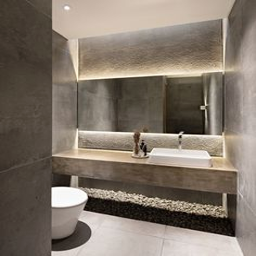
\includegraphics[width=0.25\textwidth]{assets/real_A.png}
\caption{Real Industrial bathroom (Real A)}
\label{fig:real_industrial}
\end{figure}

\begin{figure}[h]
\centering
\begin{subfigure}{0.2\textwidth}
    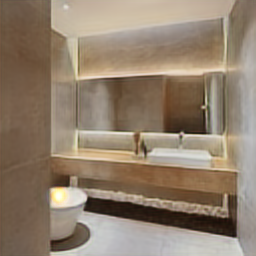
\includegraphics[width=\textwidth]{assets/fake_B.png}
    \caption{Generated Scandinavian (Fake B)}
    \label{fig:fake_scandinavian}
\end{subfigure}
\hfill
\begin{subfigure}{0.2\textwidth}
    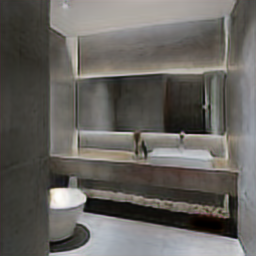
\includegraphics[width=\textwidth]{assets/rec_A.png}
    \caption{Reconstructed Industrial (Rec A)}
    \label{fig:reconstructed_industrial}
\end{subfigure}
\caption{Style transfer results from Industrial to Scandinavian and back}
\label{fig:industrial_to_scandinavian_results}
\end{figure}

Our model brightens industrial bathrooms when converting to Scandinavian style. We observe that the model seems to try to transform materials, with stone surfaces taking on wooden textures, and dark metal fixtures becoming lighter. The overall architectural structure—walls, fixtures, and general layout—is well preserved during the transformation, which is a key objective of our structural preservation loss.

\subsubsection{Scandinavian to Industrial Transfer}

Figure~\ref{fig:scandinavian_to_industrial_results} shows the transformation from scandinavian to industrial bathroom style.

\begin{figure}[h]
\centering
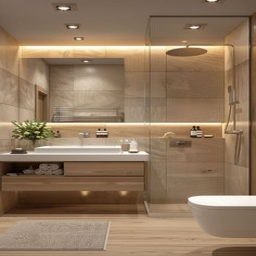
\includegraphics[width=0.2\textwidth]{assets/real_B.png}
\caption{Real Scandinavian bathroom (Real B)}
\label{fig:real_scandinavian}
\end{figure}

\begin{figure}[h]
\centering
\begin{subfigure}{0.2\textwidth}
    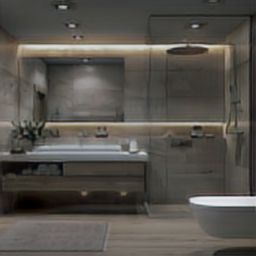
\includegraphics[width=\textwidth]{assets/fake_A.png}
    \caption{Generated Industrial (Fake A)}
    \label{fig:fake_industrial}
\end{subfigure}
\hfill
\begin{subfigure}{0.2\textwidth}
    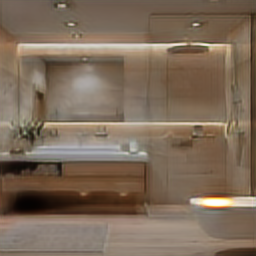
\includegraphics[width=\textwidth]{assets/rec_B.png}
    \caption{Reconstructed Scandinavian (Rec B)}
    \label{fig:reconstructed_scandinavian}
\end{subfigure}
\caption{Style transfer results from Scandinavian to Industrial and back}
\label{fig:scandinavian_to_industrial_results}
\end{figure}

When converting from Scandinavian to Industrial style, our model creates darker tones, sometimes approaching a black and white aesthetic. The model seems to be adding bronze-like materials or anthracite grey/black accents to sinks and mirror borders. This subtlety may be attributed to the model's focus on preserving structural elements while changing stylistic features.

\subsection{Cycle Consistency Analysis}

Figure~\ref{fig:cycle_consistency} illustrates the full cycle of transformations for both directions.

\begin{figure}[h]
\centering
% Replace with actual path to your best sample image
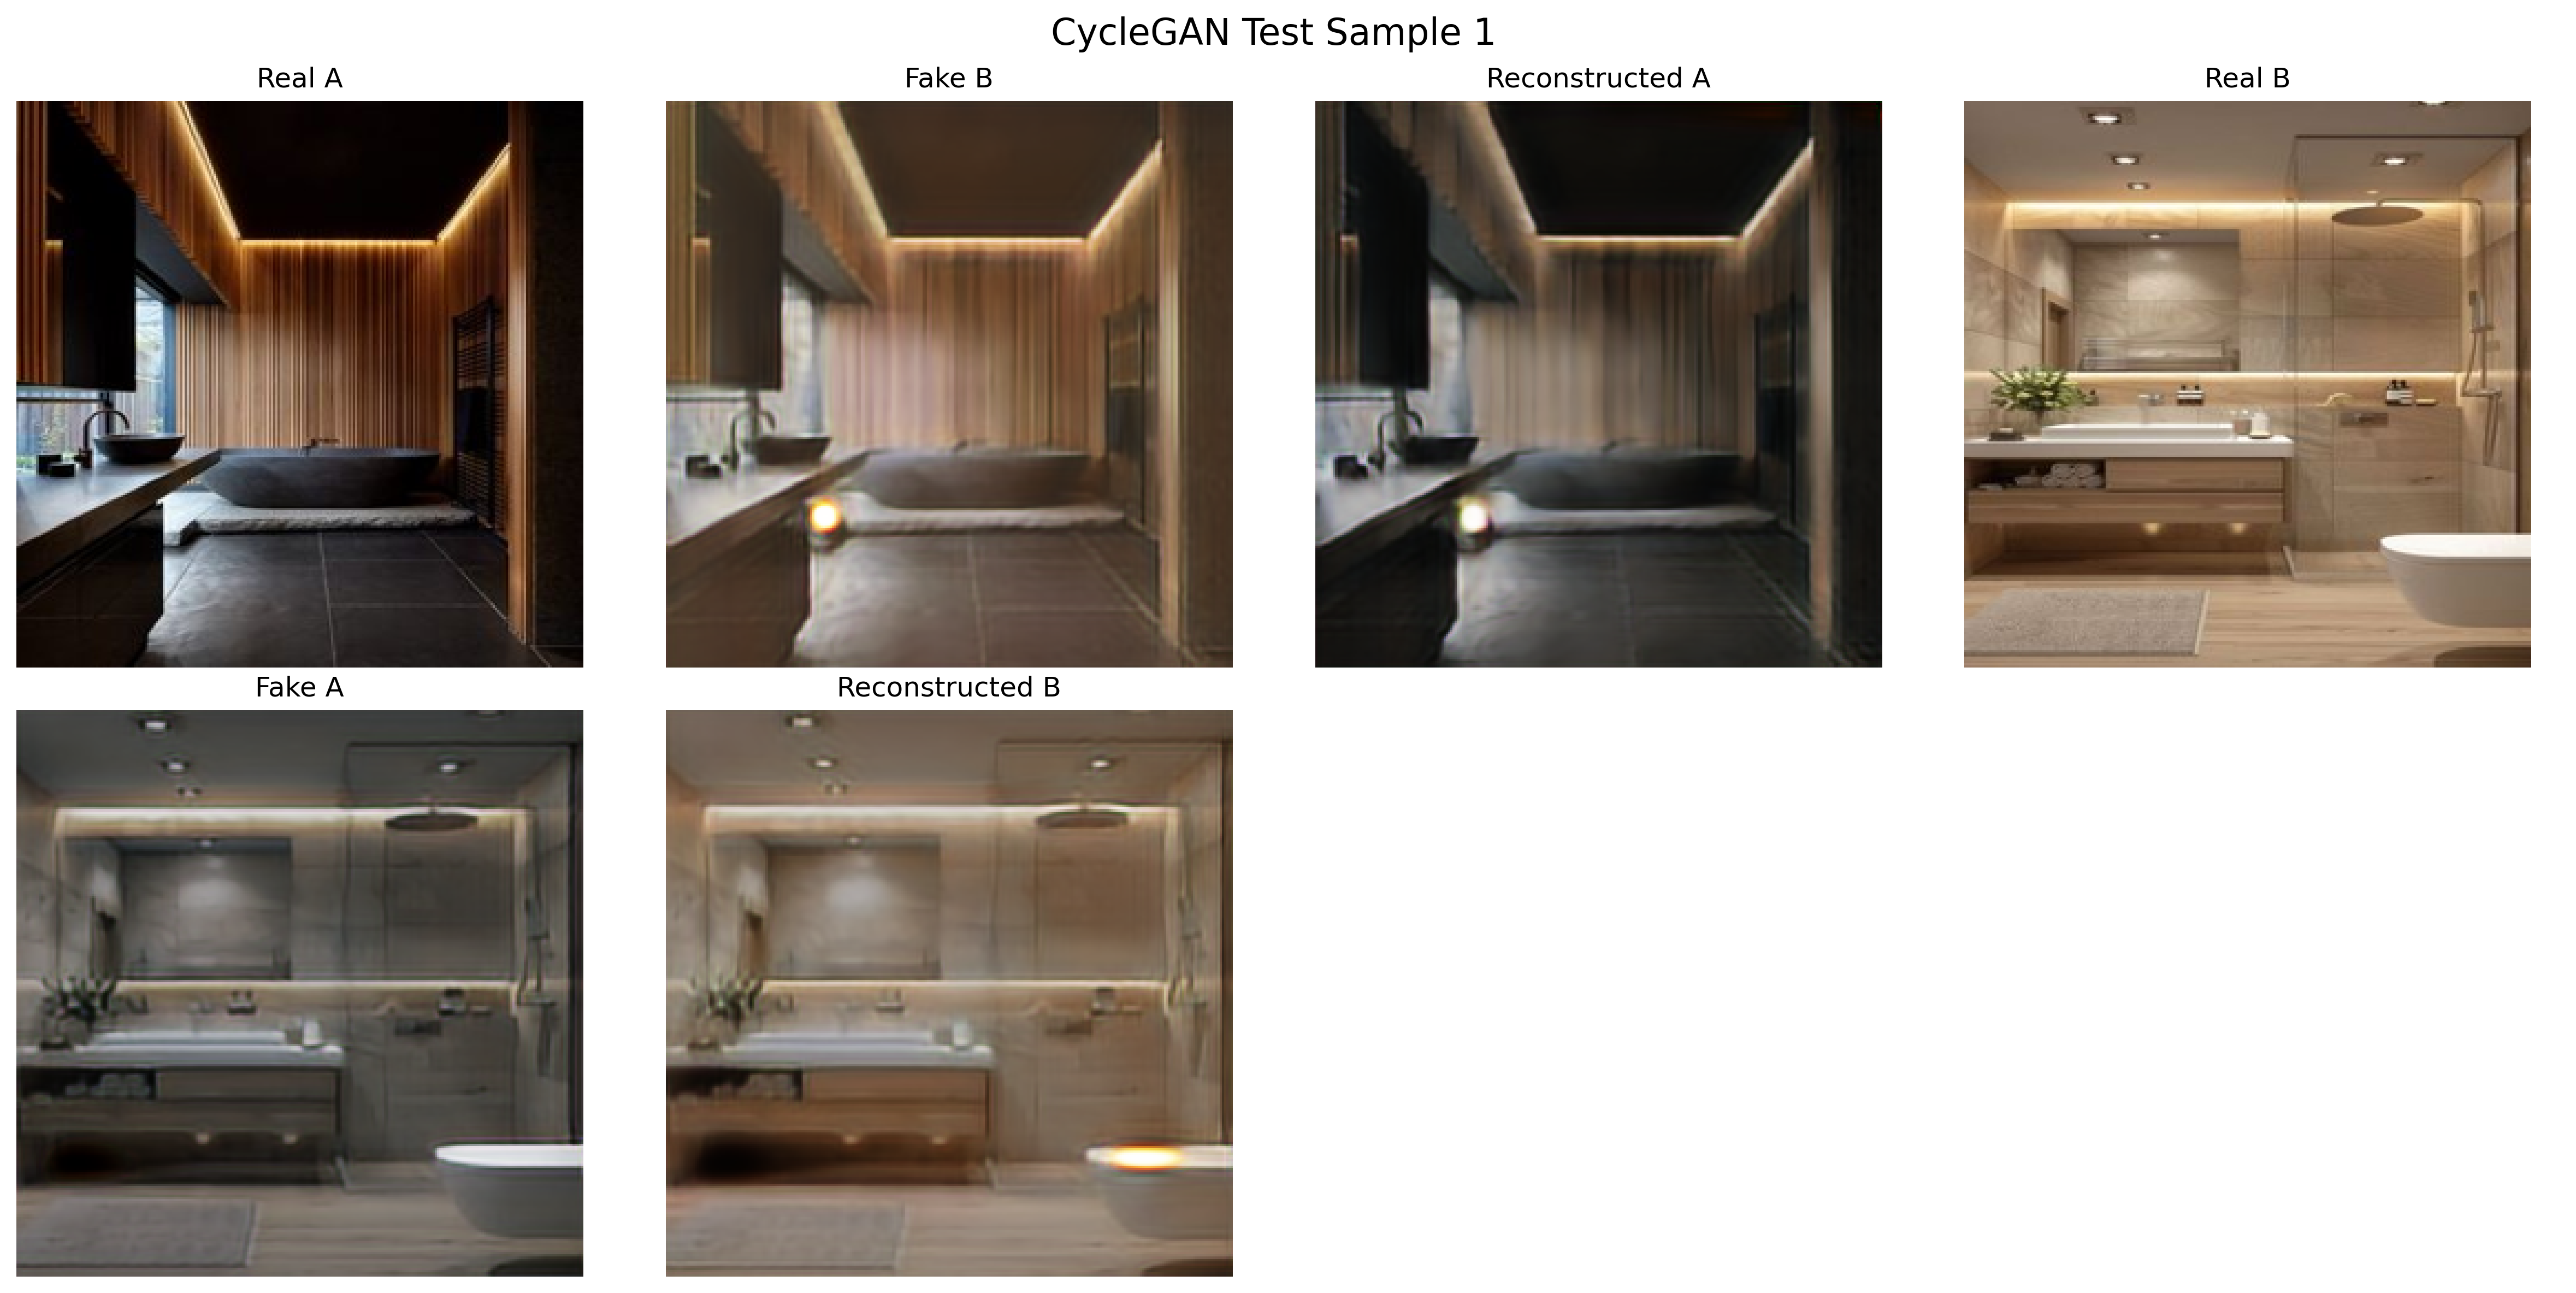
\includegraphics[width=0.5\textwidth]{assets/sample_1.png}
\caption{Complete style transfer cycles. Industrial → Scandinavian → Industrial. Scandinavian → Industrial → Scandinavian.}
\label{fig:cycle_consistency}
\end{figure}

The cycle consistency results show that after a full transformation cycle, images return to a state visually similar to their originals. For the Industrial → Scandinavian → Industrial cycle, the reconstructed image recovers the darker tones, while for the Scandinavian → Industrial → Scandinavian cycle, the model successfully retrieves the brighter aesthetic of Scandinavian design.

\subsection{Structural Preservation}

A key feature of our approach is the structural preservation loss, which aims to maintain architectural elements while allowing stylistic changes. As visible in Figures~\ref{fig:industrial_to_scandinavian_results} and \ref{fig:scandinavian_to_industrial_results}, our model preserves the bathroom layout, fixture positions, and architectural boundaries while transforming the atmosphere, tones and sometimes materials. \\

The LPIPS structural scores (0.2620 for A to B and 0.2163 for B to A) support our visual observation that structural elements are largely preserved during style transfer. The better score for Scandinavian to Industrial transformation suggests that preserving structure while darkening and adding industrial textures may be easier than the reverse process. This asymmetry could be due to the nature of Scandinavian design, which often features simpler, cleaner lines that provide less structural information compared to the more complex textures and fixtures often found in industrial bathrooms. \\

Looking at the transformation examples, we can observe that elements positions and forms remain consistent through the style transfer process, while surface materials, color palettes, and lights are modified to match the target aesthetic. This shows the effectiveness of our structural preservation loss in guiding the model to distinguish between content that should be preserved and stylistic elements that should be transformed.

\section{Discussion}

While our CycleGAN approach produces promising results, our project has several limitations that require critical examination.

\subsection{Limitations of Style Transfer for Interior Design}

Our experiments demonstrate that the current approach can effectively transform certain stylistic elements like colors, textures, and material appearances, but falls short in making more substantial changes that may be desired in interior design contexts. The model primarily alters the "atmosphere" of the bathrooms—brightening spaces when converting to Scandinavian style or darkening them for Industrial style—but struggles with more meaningful transformations. \\

The high FID scores (average of 192.78) indicate a significant distribution gap between generated and real images, suggesting that our transformations are not fully capturing the authentic characteristics of each design style. This limitation may stem from both the model architecture and the relatively small dataset size.

\subsection{Insufficient Feature Engineering}

One shortcoming of our implementation is the minimal feature engineering. While we adopted Fu's enhanced CycleGAN architecture, we did not develop domain-specific features tailored to interior design. For example:

\begin{itemize}
    \item No semantic segmentation to distinguish between different bathroom elements (walls, fixtures, floor, etc.)
    \item Lack of material-specific transformations that could better capture design style differences
    \item No specialized attention mechanisms to focus on style-defining elements
    \item Absence of design-specific perceptual features for more meaningful loss functions
\end{itemize}

These limitations restrict the model's ability to make targeted, design-relevant transformations, instead producing more general stylistic changes.

\subsection{Structural Preservation vs. Design Transformation}

Perhaps the most significant limitation lies in our adherence to structural preservation. While Fu's approach made sense for artwork where preserving the composition was essential, interior design transformation often requires changes to furniture and fixtures. Our strong structural preservation loss forces the model to maintain all architectural elements, preventing it from:

\begin{itemize}
    \item Replacing industrial metal fixtures with wooden Scandinavian alternatives
    \item Transforming bathtub designs between styles
    \item Changing sink shapes and materials in a style-appropriate manner
    \item Modifying lighting fixtures which are key style indicators
\end{itemize}

This reveals a fundamental tension in our approach: successful interior style transfer often requires structural changes, yet our model explicitly penalizes such modifications. This constraint significantly limits the practical utility of the system for design visualization.

\subsection{CycleGAN Limitations for Design Applications}

Our results suggest that CycleGAN, even with enhancements, may not be the optimal architecture for sophisticated interior design transformations. The inherent limitations include:

\begin{itemize}
    \item Inability to generate new elements not present in the original image
    \item Limited capacity to understand the semantic meaning of different room components
    \item Tendency to produce artifacts in complex regions with many geometric details
\end{itemize}

These architectural limitations are evident in our results, where style transfer is largely limited to color shifts and texture changes rather than meaningful design transformations.

\subsection{Alternative Approaches}

The limitations identified suggest that newer generative models, particularly diffusion models, might be better suited for interior design style transfer. Recent text-to-image and image-to-image diffusion models such as Stable Diffusion have shown superior capabilities in:

\begin{itemize}
    \item Understanding semantic content of scenes
    \item Generating new objects and elements while maintaining context
    \item Producing high-fidelity transformations guided by text prompts
    \item Preserving important elements while allowing for targeted modifications
\end{itemize}

A diffusion-based approach would potentially allow for both preservation of room structure and transformation of specific design elements through controlled generation. This could enable more meaningful style transfers that actually replace industrial fixtures with Scandinavian ones, rather than merely adjusting their appearance. \\

Furthermore, we could also address the fundamental limitation of our current system, which applies the same transformation logic to all bathroom elements regardless of their design significance.

\section{Conclusion and Future Work}

In this paper, we presented a deep learning approach for bathroom interior design style transfer using an enhanced CycleGAN architecture. Our system transforms bathroom images between industrial and scandinavian styles, changing the atmosphere and material appearances while preserving the room structure. The quantitative results, with LPIPS cycle consistency scores around 0.25, show that our model achieves a reasonable balance between style transformation and content preservation. Our visual results confirm this finding, showing clear stylistic changes from dark, metallic industrial aesthetics to bright, clean scandinavian designs and vice versa. The multi-scale discriminator and structural preservation loss were valuable in maintaining architectural integrity throughout these transformations. \\

Despite these achievements, our approach has limitations in making substantial furniture and fixture modifications necessary for complete style transformations. Future work should incorporate semantic understanding of room elements to enable more targeted transformations, potentially allowing specific fixtures to be redesigned while maintaining overall room structure. Additionally, exploring more advanced generative models, such as diffusion-based approaches, could overcome the limitations of CycleGAN and enable more sophisticated interior design transformations with improved fidelity. As a conclusion, while our current system shows the feasibility of automated room style transfer, the path toward truly comprehensive design visualization will require these more nuanced approaches that better balance preservation and transformation.


% ==============================================================================

\appendix
\section{Training Visualizations}

This appendix contains the complete set of training visualization charts generated during our model training process. These visualizations were captured using Weights \& Biases (wandb) monitoring tool over the course of 100 epochs.

\subsection{Overall Loss Charts}

\begin{figure}[H]
\centering
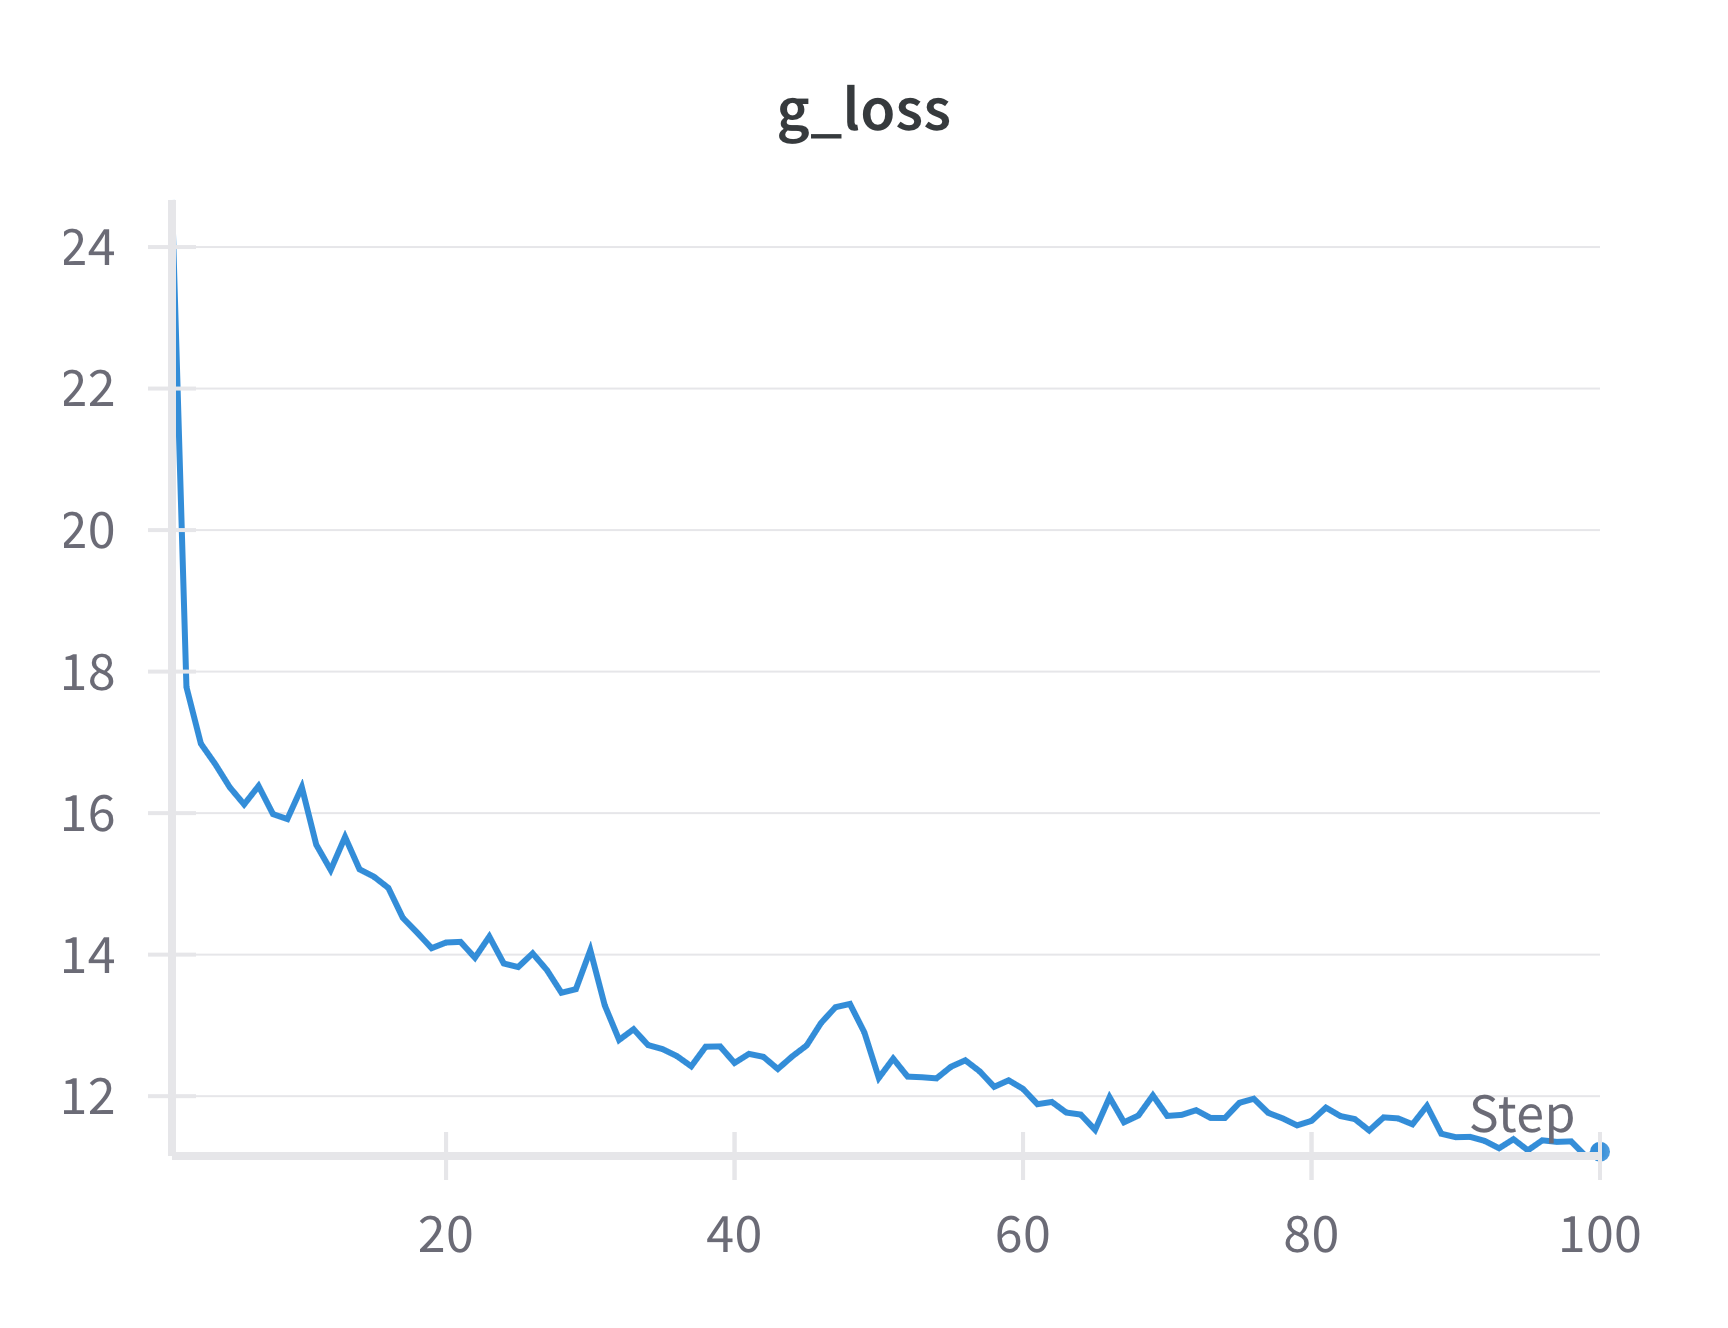
\includegraphics[width=0.45\textwidth]{assets/g_loss.png}
\caption{Generator loss (g\_loss)}
\label{fig:g_loss}
\end{figure}

\begin{figure}[H]
\centering
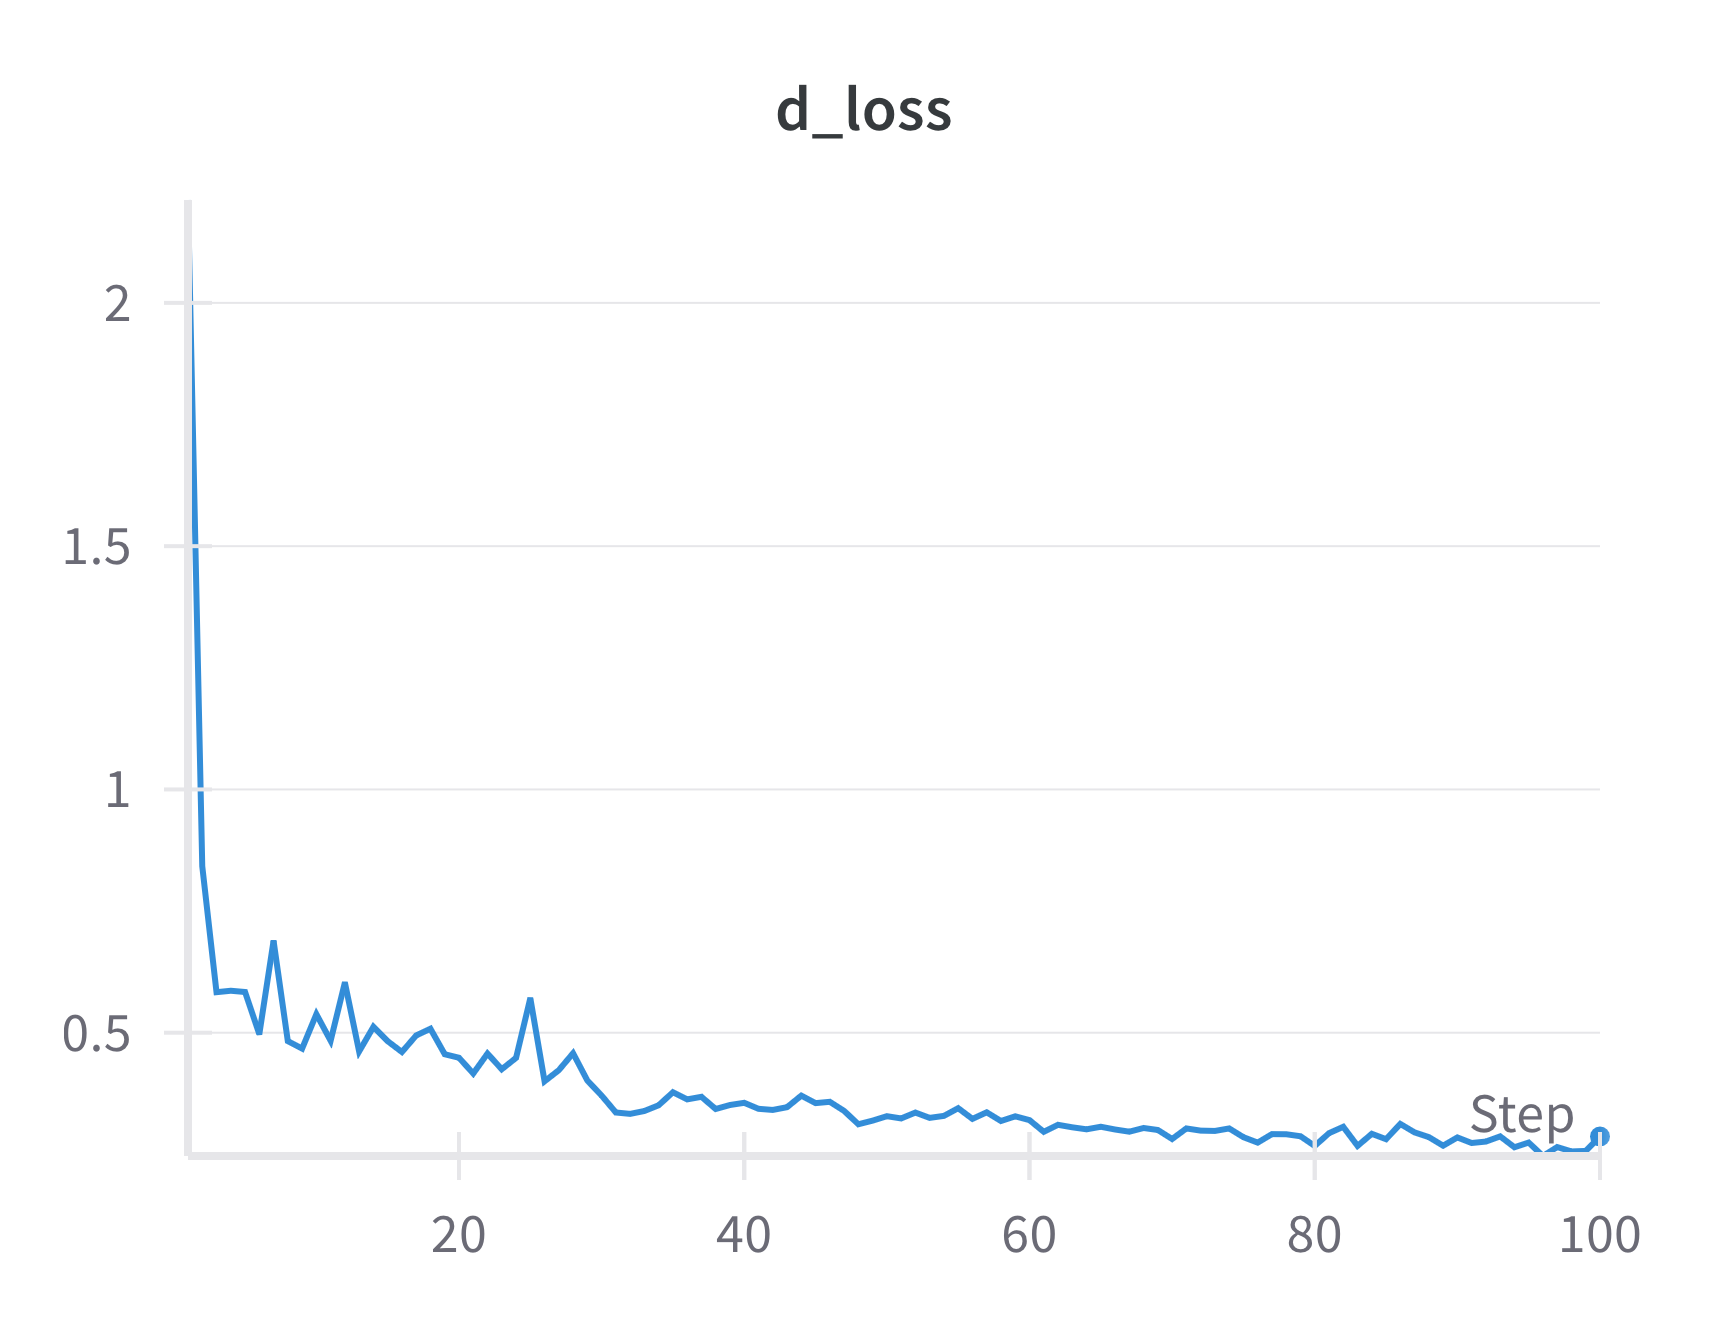
\includegraphics[width=0.45\textwidth]{assets/d_loss.png}
\caption{Discriminator loss (d\_loss)}
\label{fig:d_loss}
\end{figure}

\begin{figure}[H]
\centering
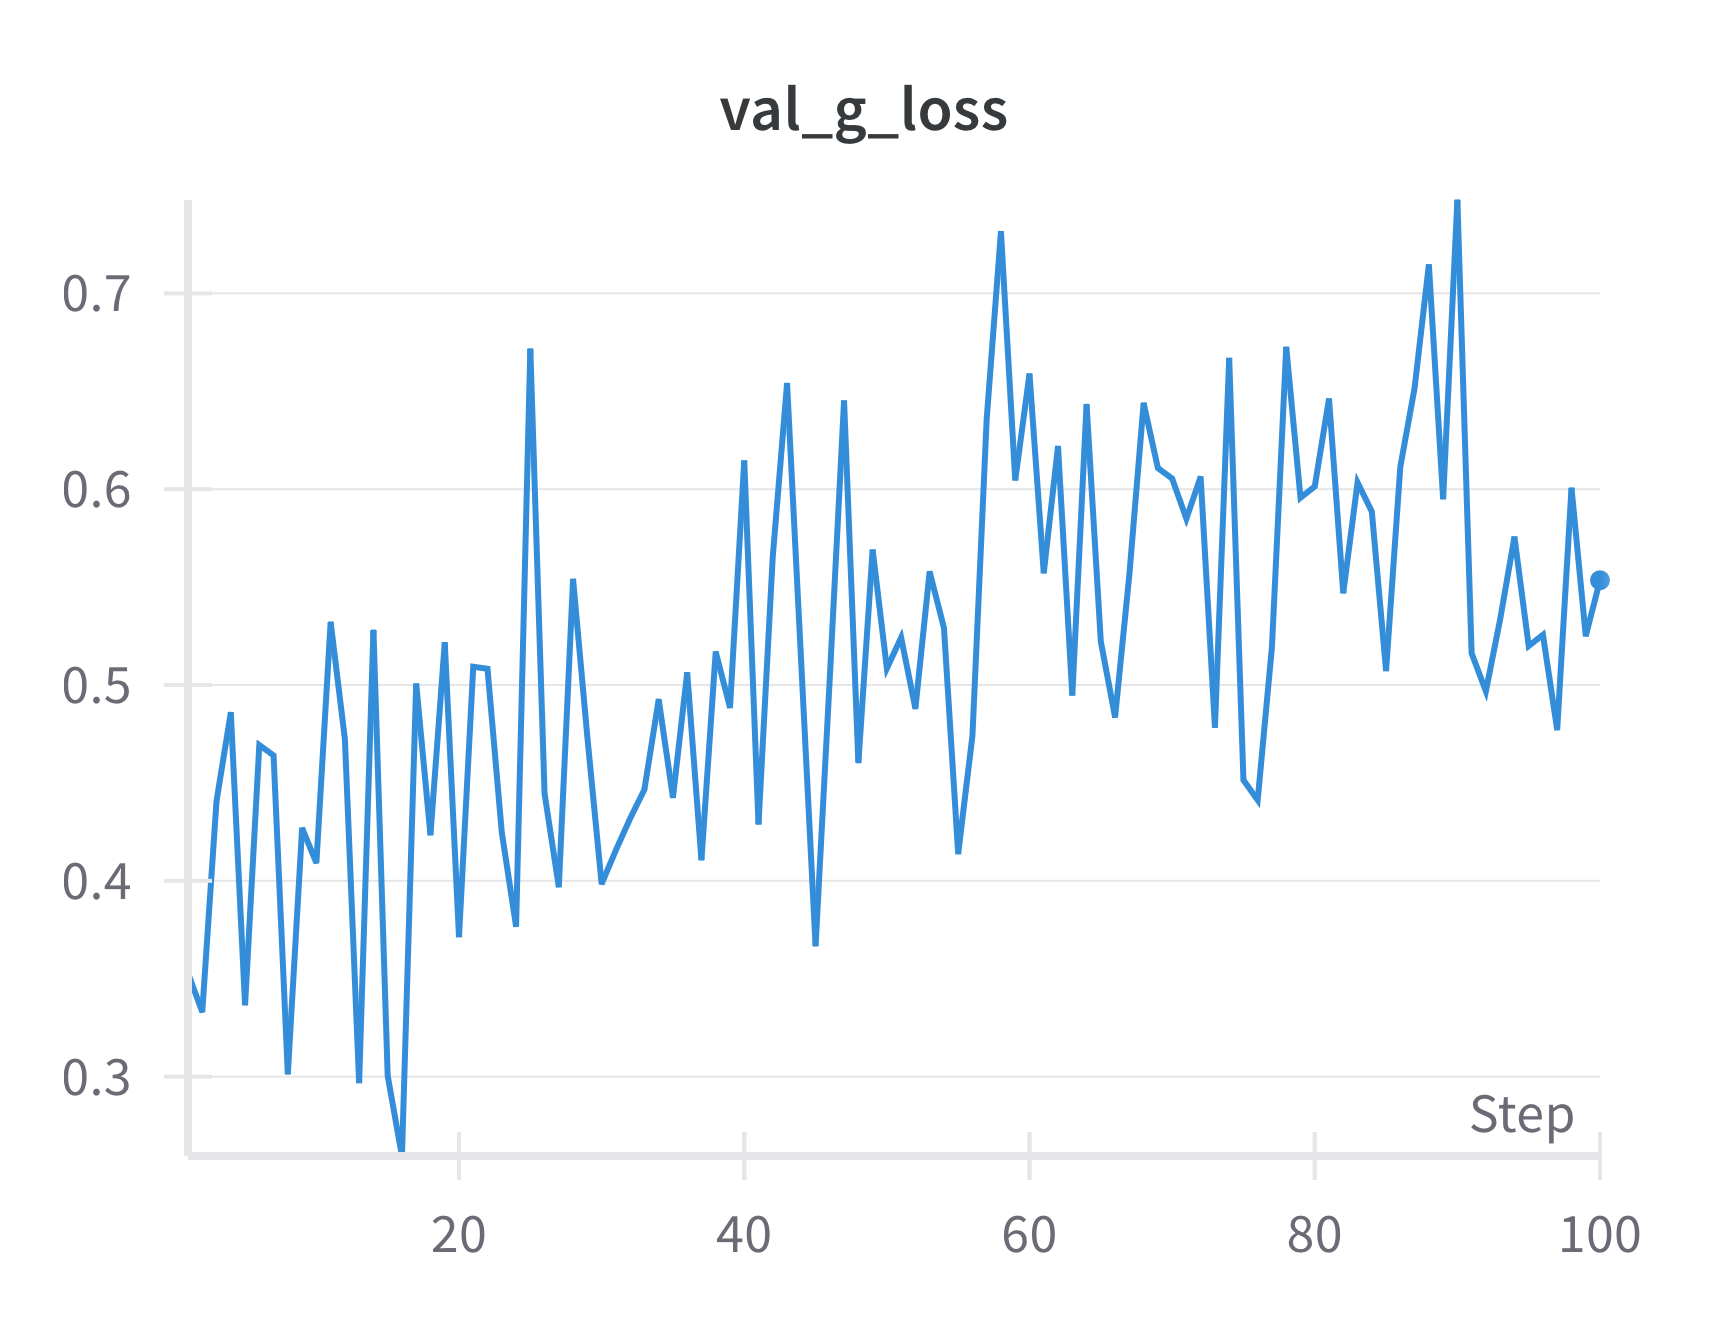
\includegraphics[width=0.45\textwidth]{assets/val_g_loss.png}
\caption{Validation generator loss (val\_g\_loss)}
\label{fig:val_g_loss}
\end{figure}

\begin{figure}[H]
\centering
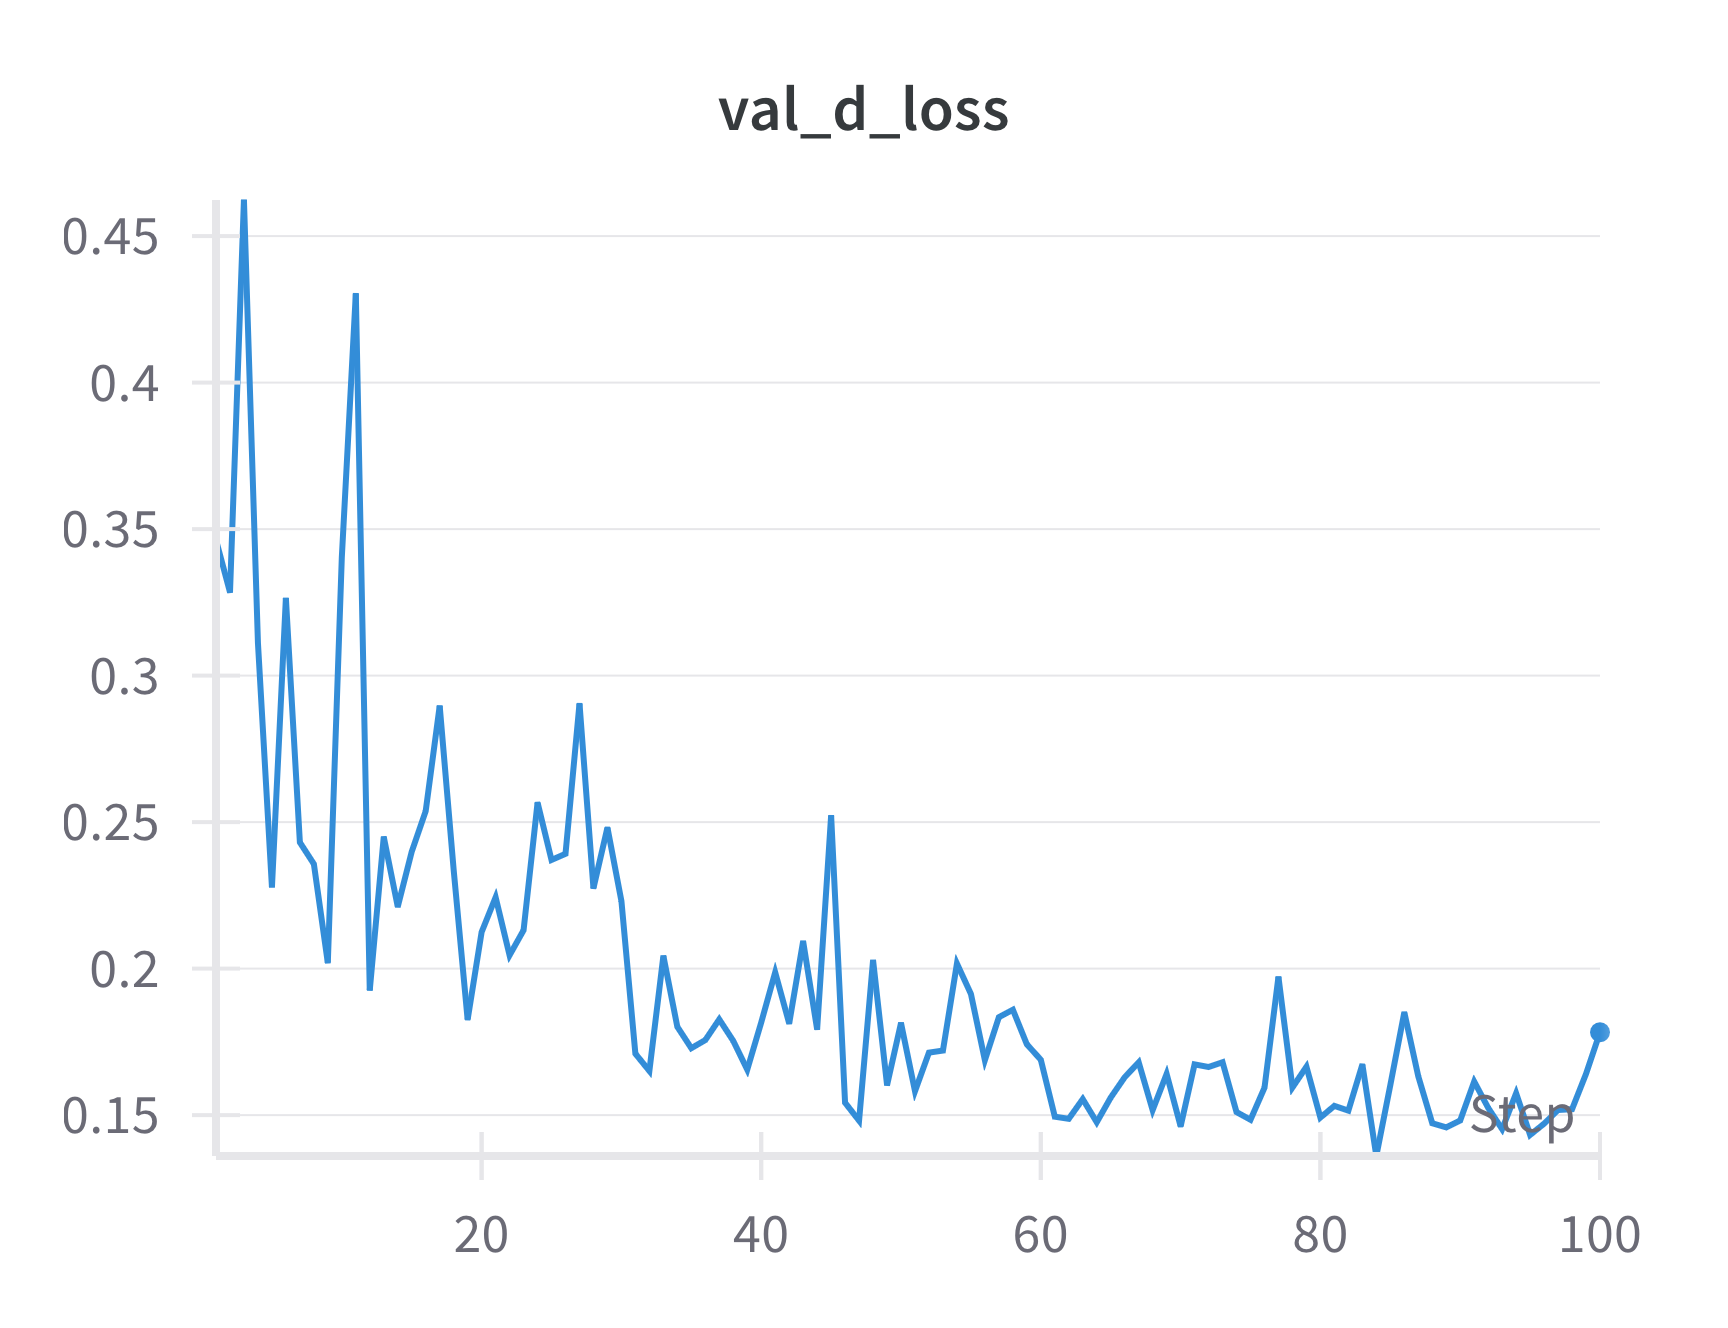
\includegraphics[width=0.45\textwidth]{assets/val_d_loss.png}
\caption{Validation discriminator loss (val\_d\_loss)}
\label{fig:val_d_loss}
\end{figure}

\subsection{Learning Rate Schedule}

\begin{figure}[H]
\centering
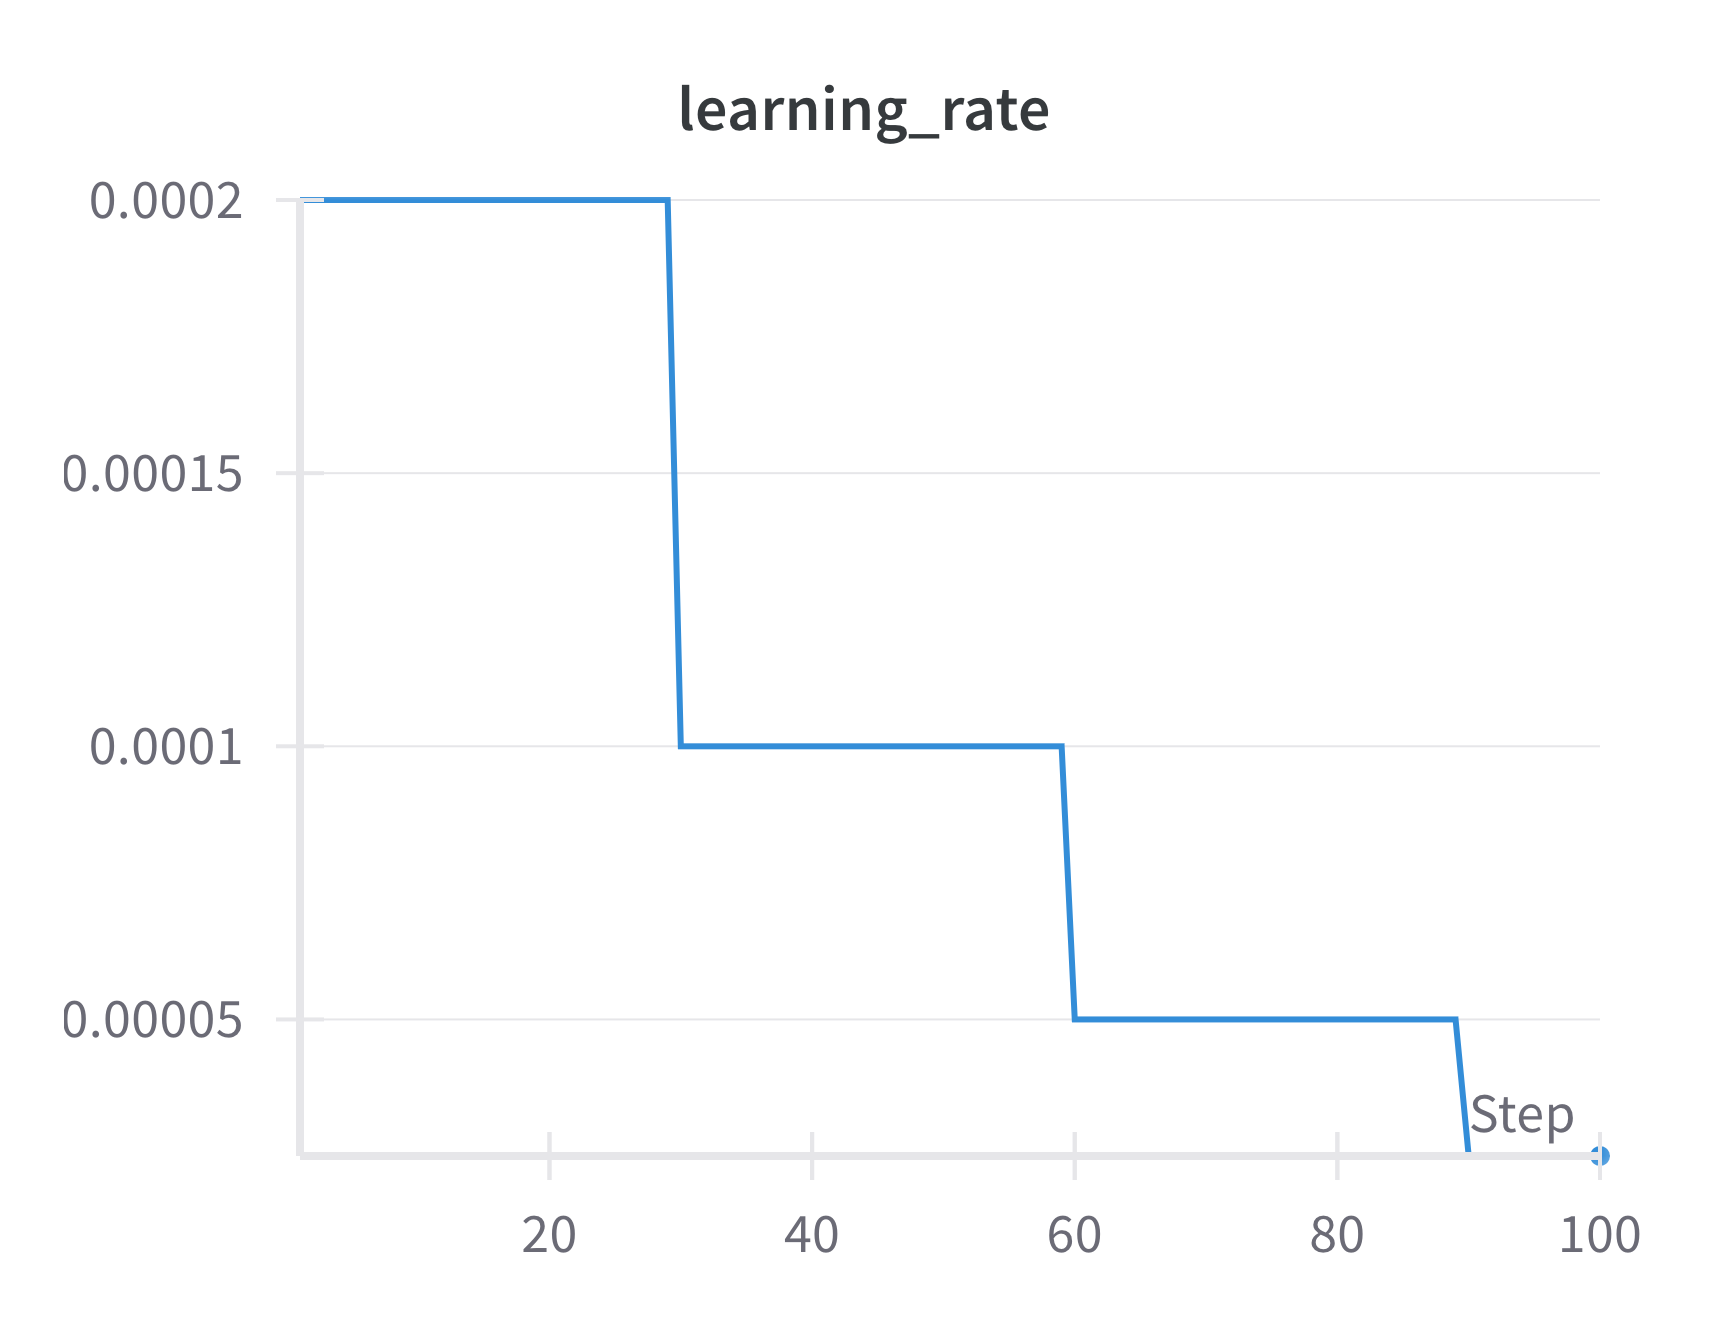
\includegraphics[width=0.45\textwidth]{assets/learning_rate.png}
\caption{Learning rate}
\label{fig:learning_rate}
\end{figure}

\subsection{Domain-Specific Adversarial Losses}

\begin{figure}[H]
\centering
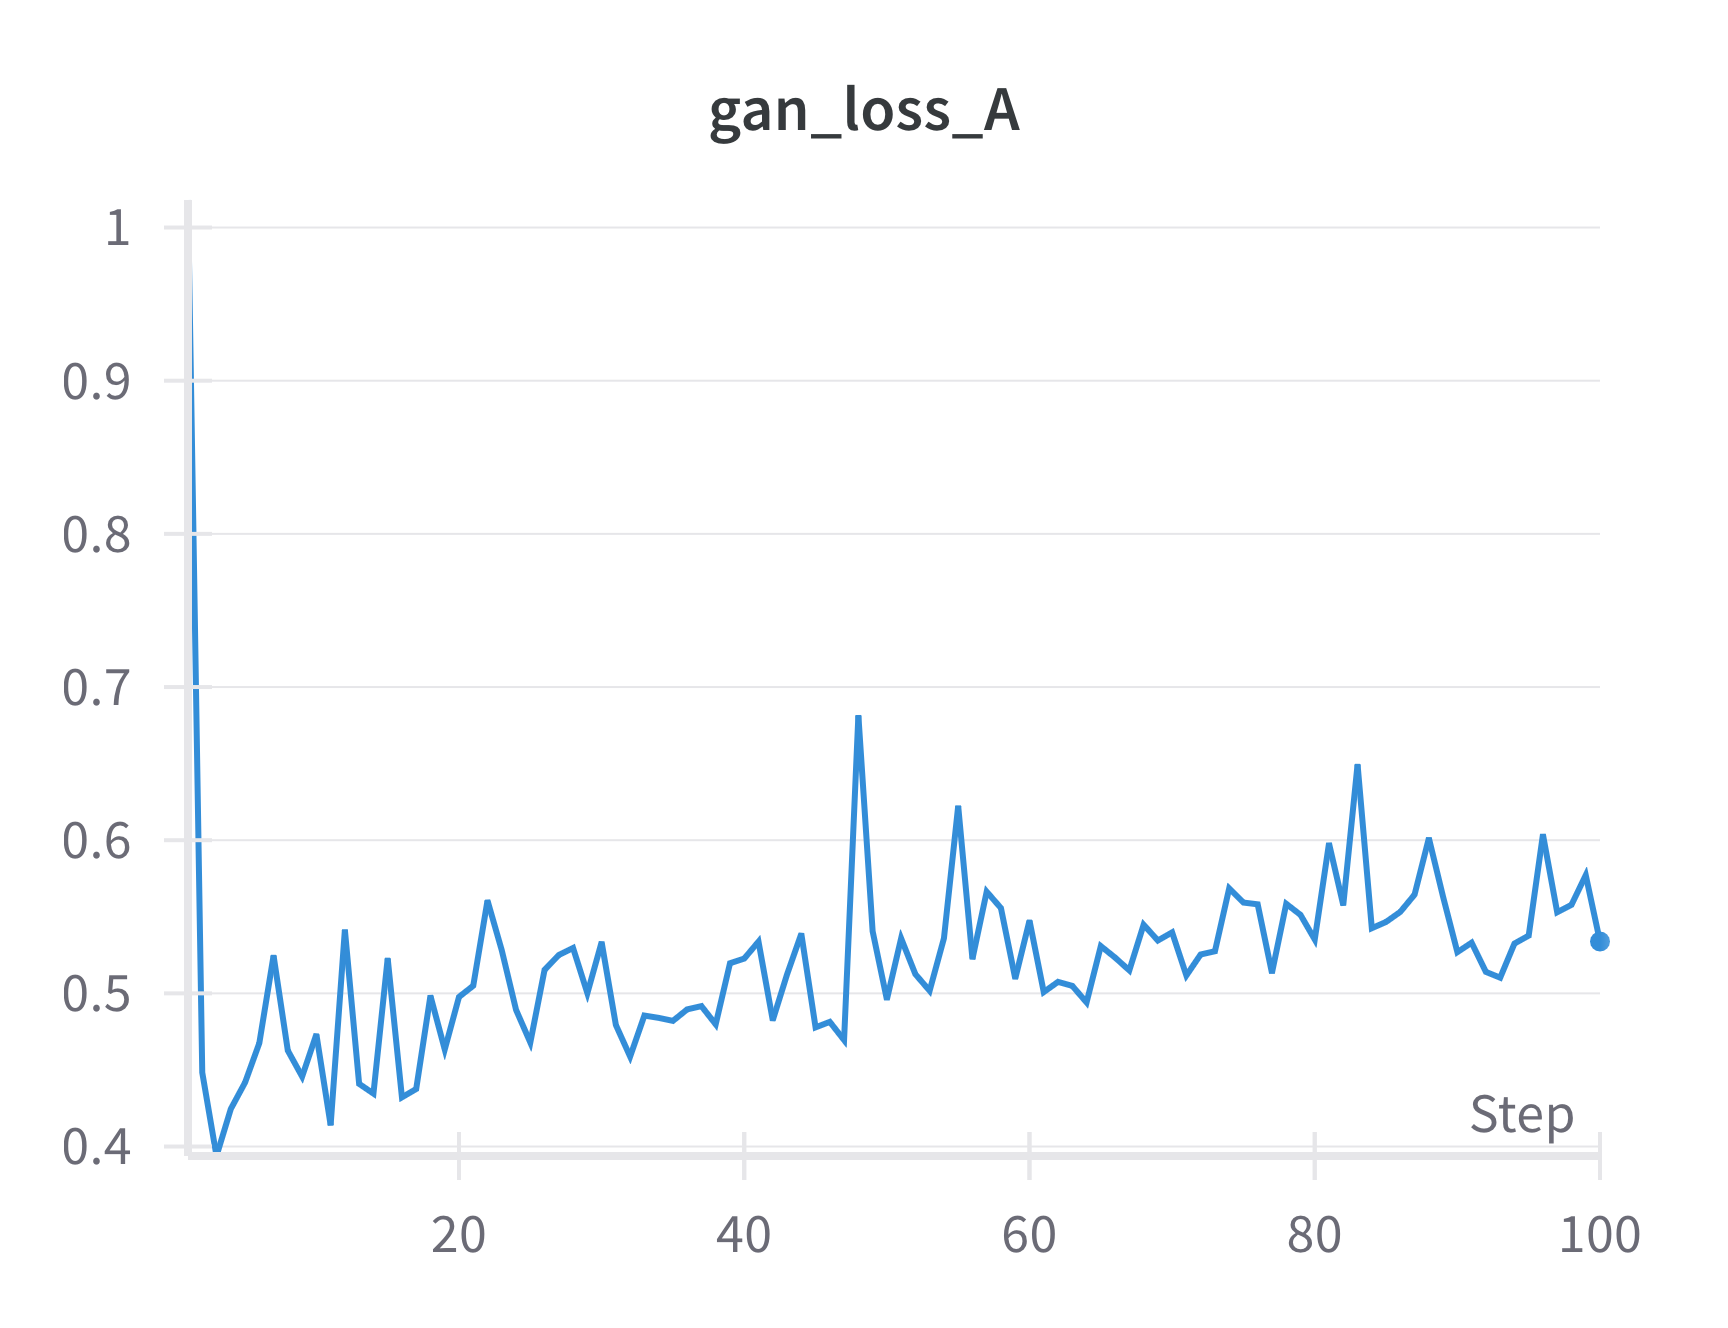
\includegraphics[width=0.45\textwidth]{assets/gan_loss_A.png}
\caption{GAN adversarial loss for domain A (gan\_loss\_A)}
\label{fig:gan_loss_A}
\end{figure}

\begin{figure}[H]
\centering
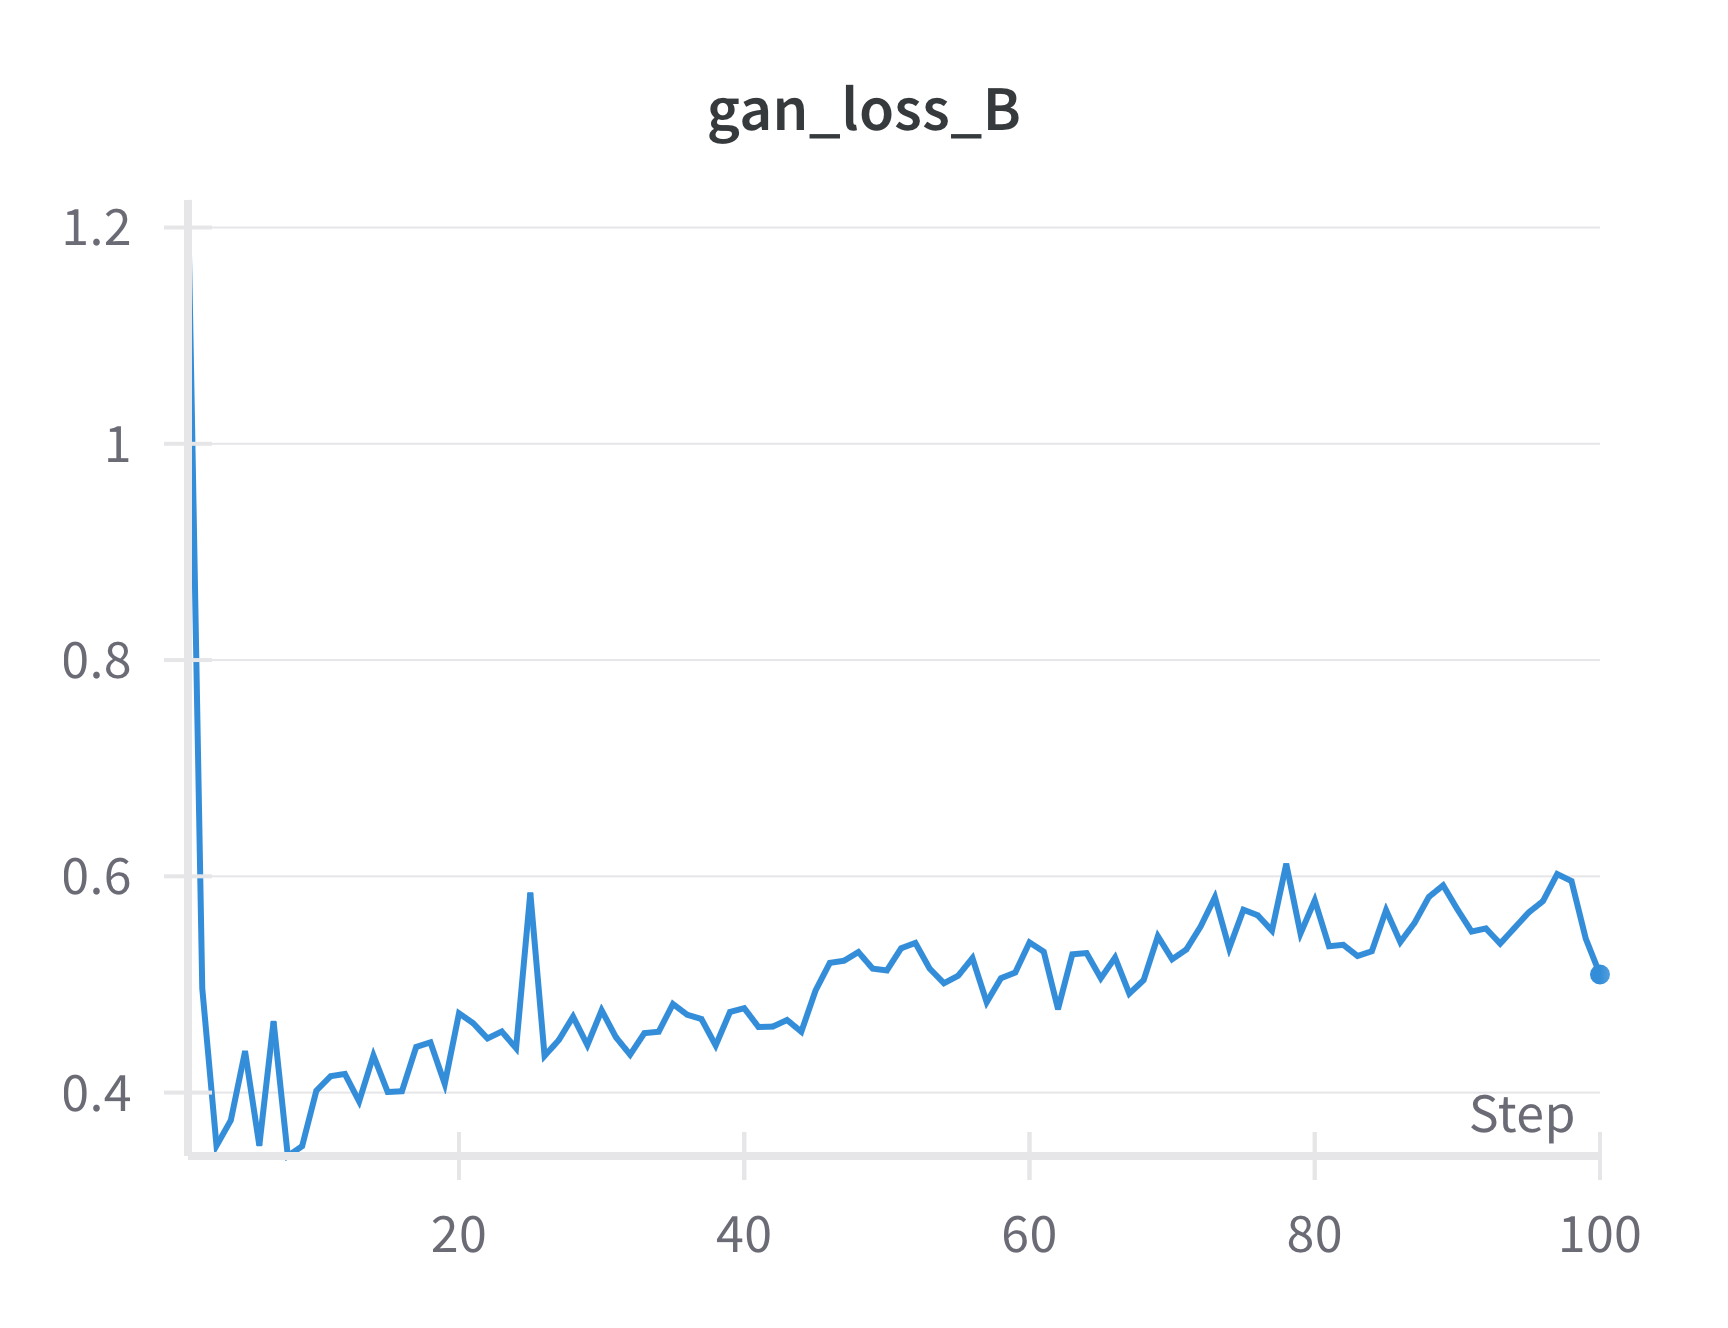
\includegraphics[width=0.45\textwidth]{assets/gan_loss_B.png}
\caption{GAN adversarial loss for domain B (gan\_loss\_B)}
\label{fig:gan_loss_B}
\end{figure}

\begin{figure}[H]
\centering
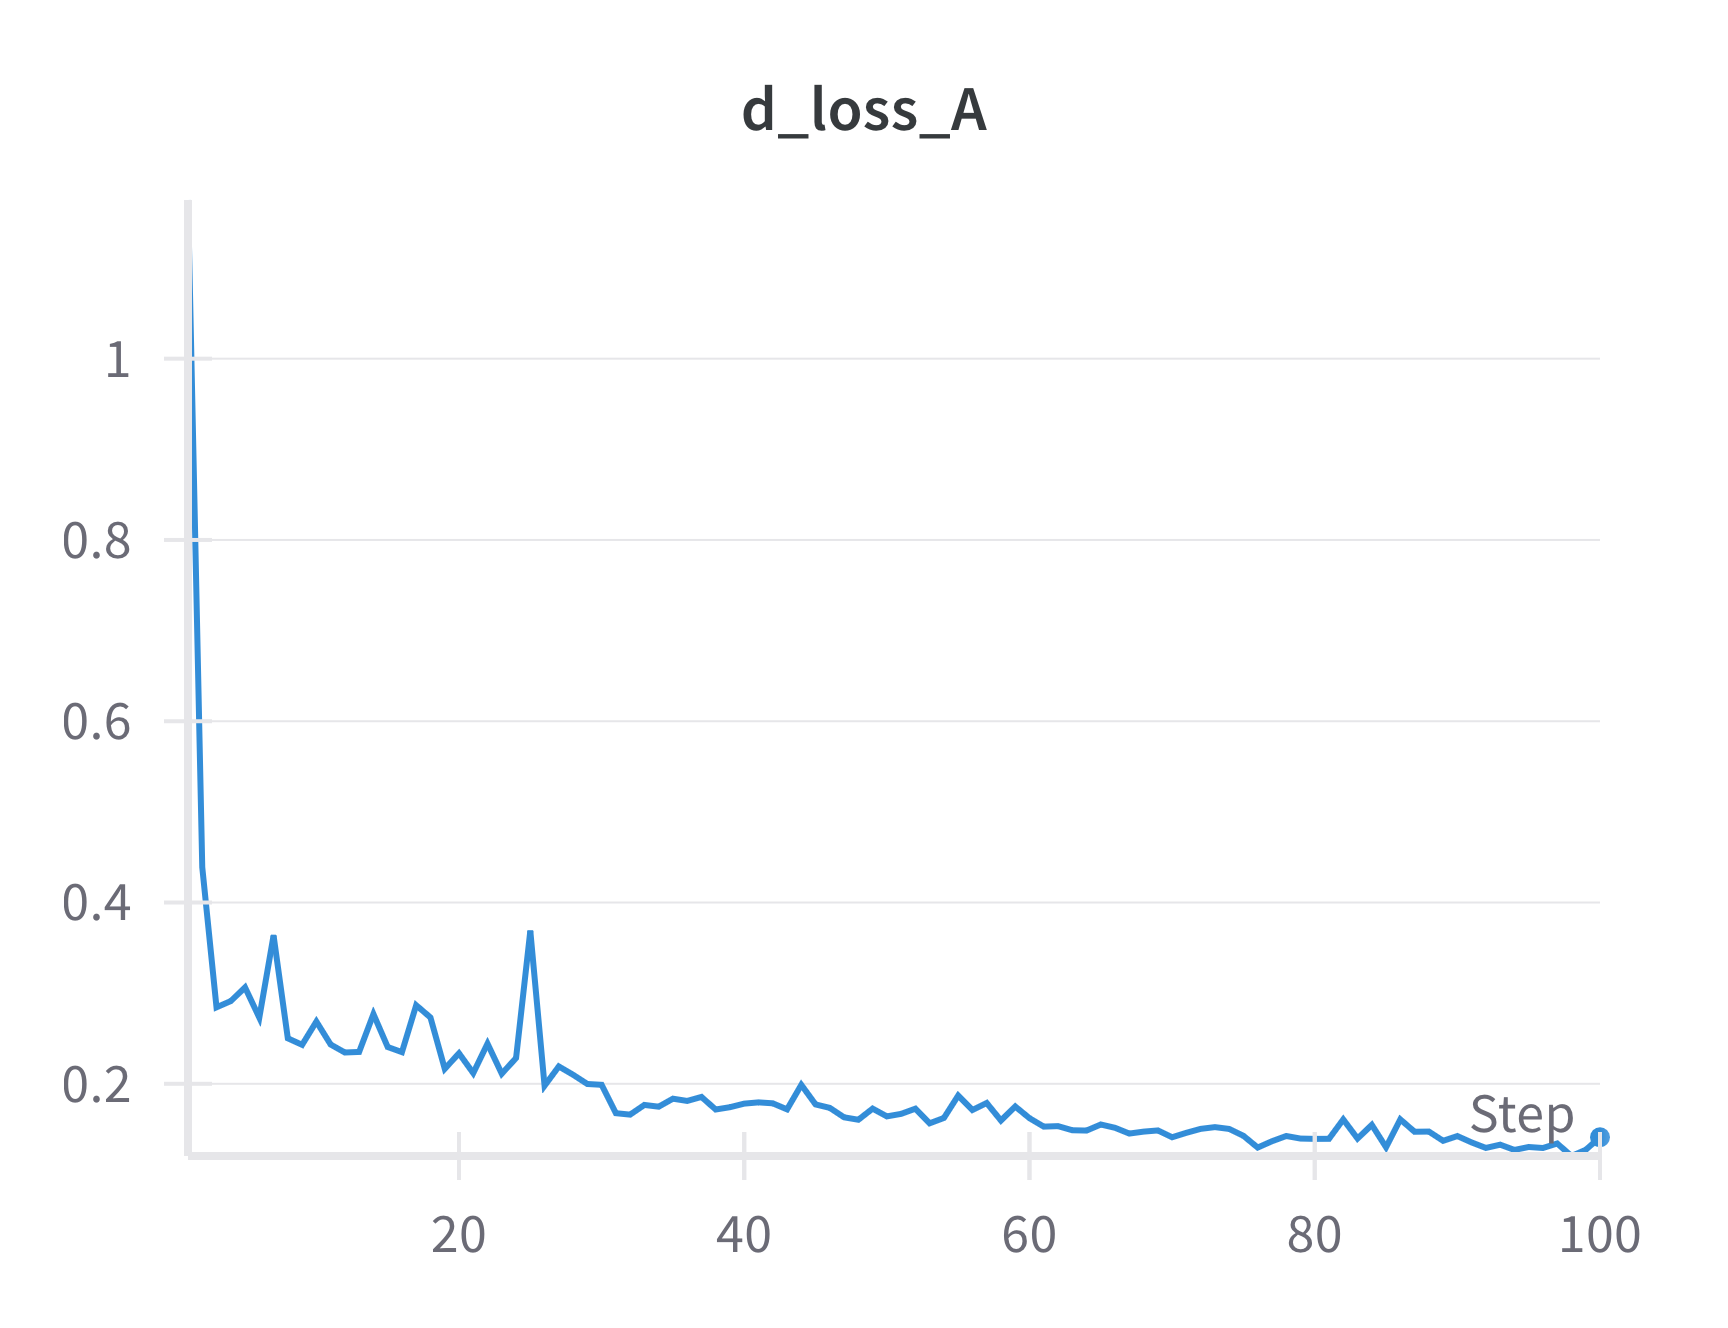
\includegraphics[width=0.45\textwidth]{assets/d_loss_A.png}
\caption{Discriminator loss for domain A (d\_loss\_A)}
\label{fig:d_loss_A}
\end{figure}

\begin{figure}[H]
\centering
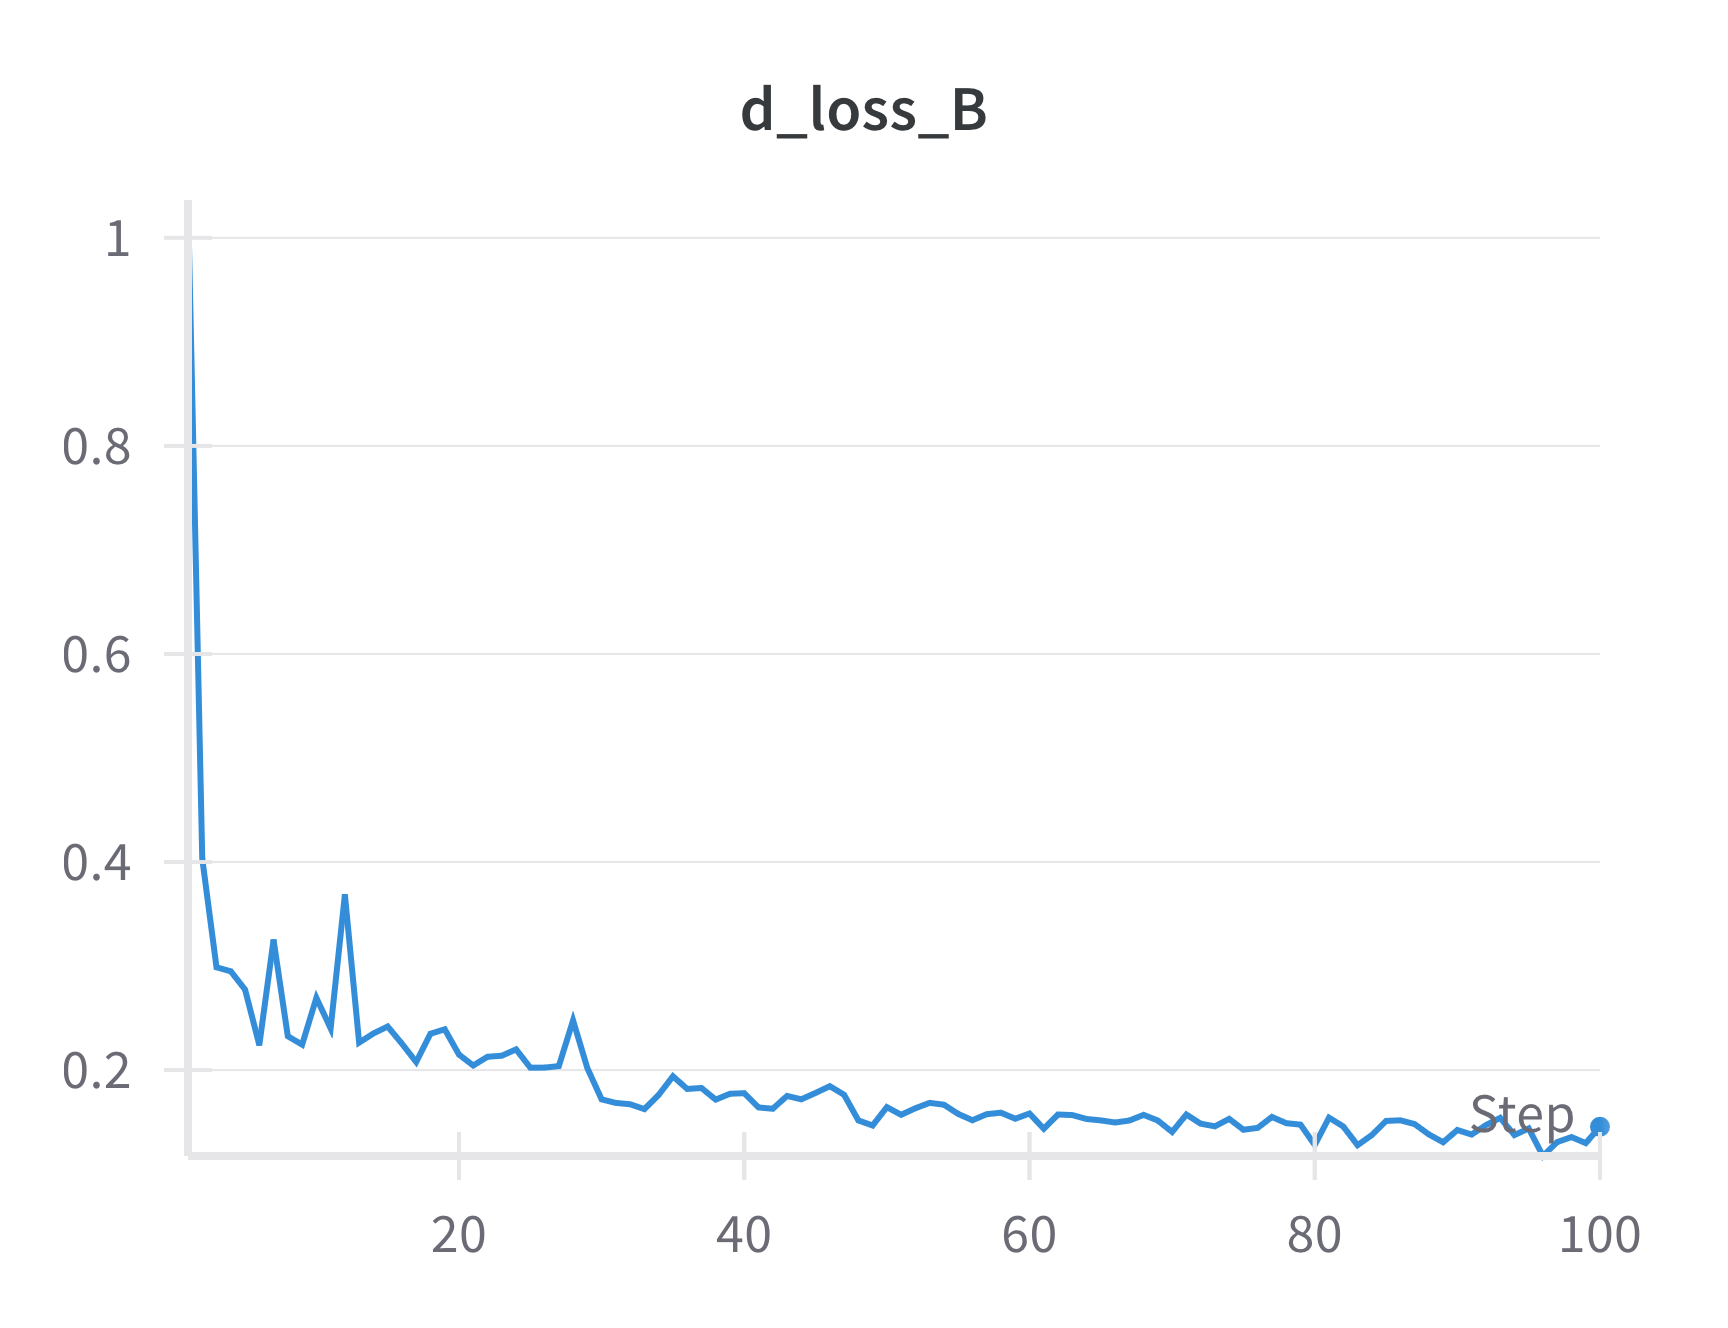
\includegraphics[width=0.45\textwidth]{assets/d_loss_B.png}
\caption{Discriminator loss for domain B (d\_loss\_B)}
\label{fig:d_loss_B}
\end{figure}

\subsection{Cycle Consistency and Structural Preservation Losses}

\begin{figure}[H]
\centering
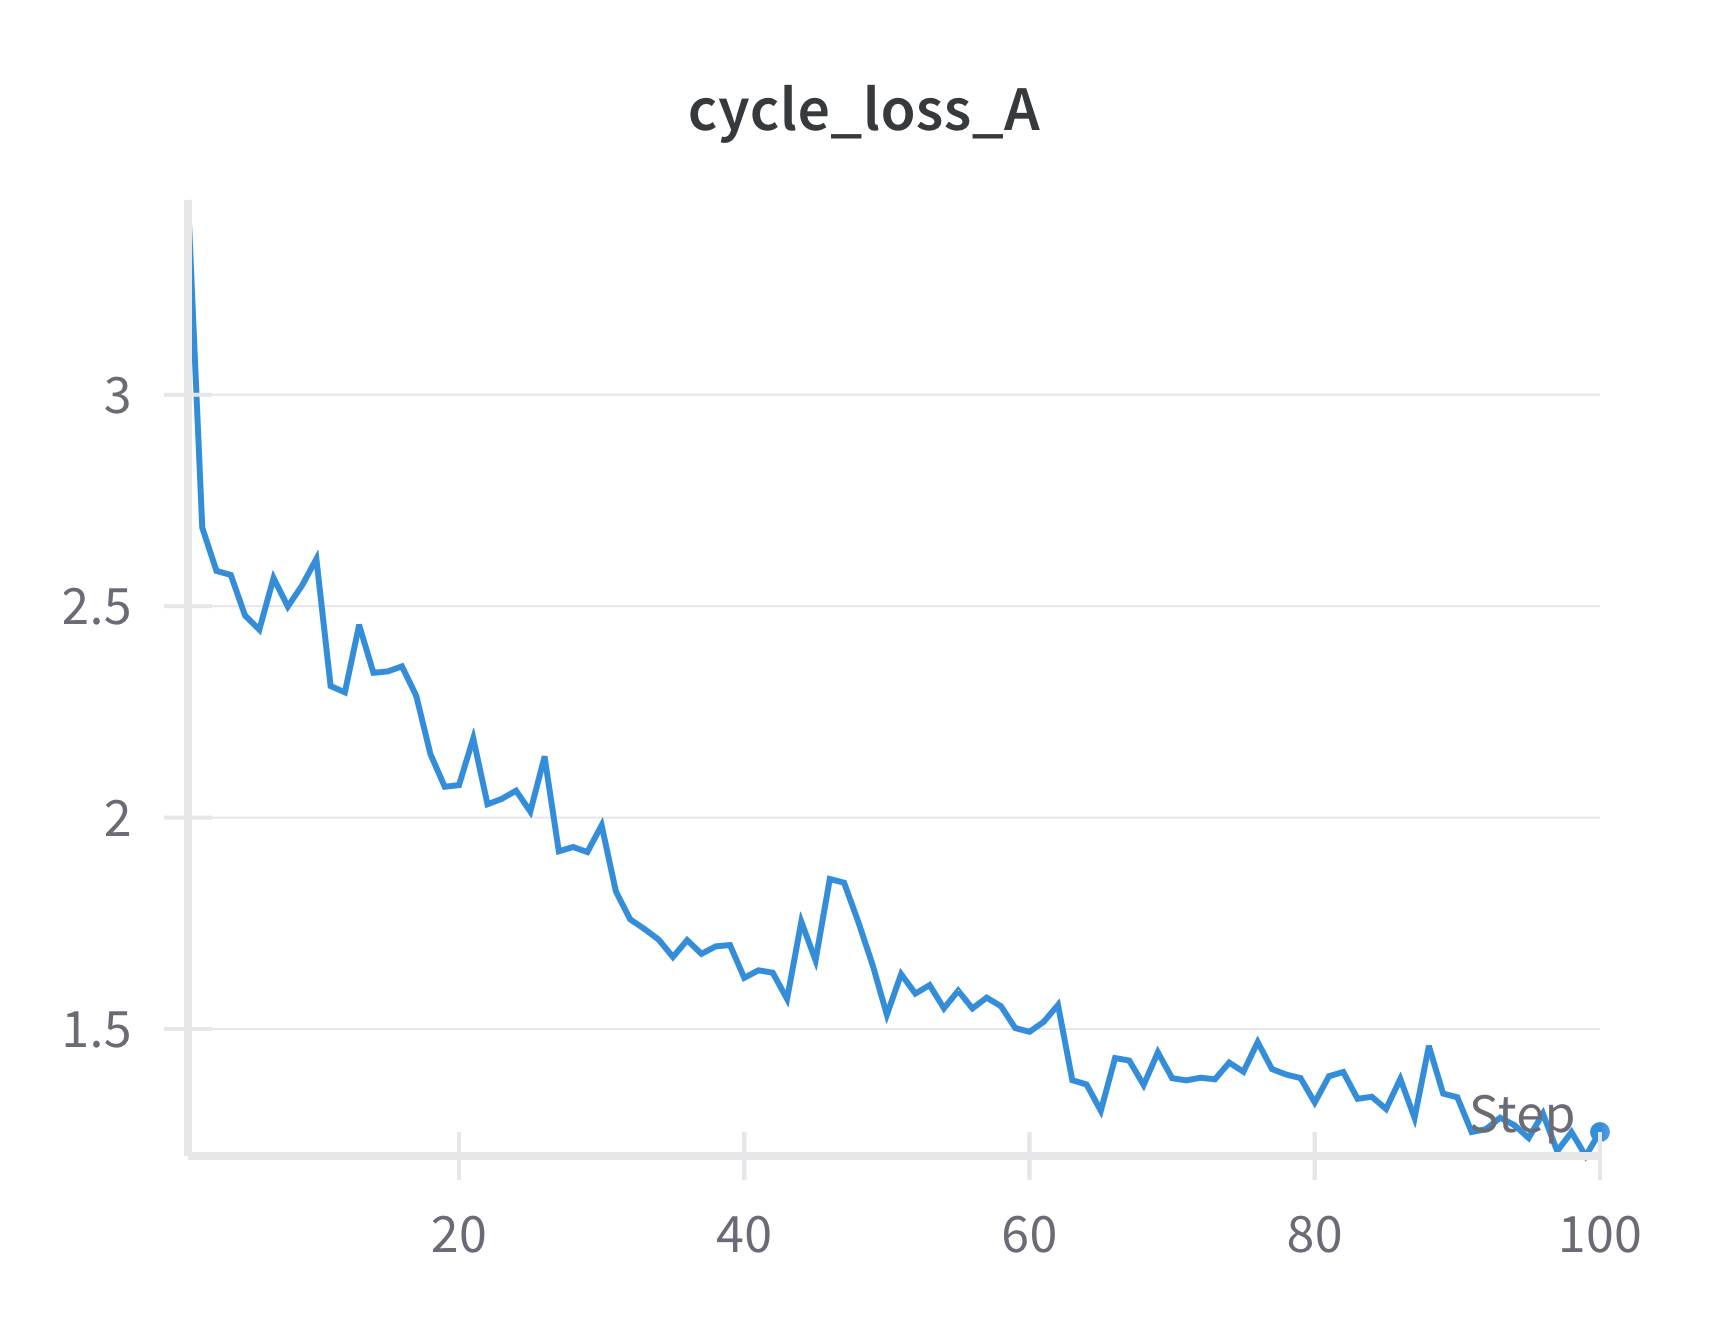
\includegraphics[width=0.45\textwidth]{assets/cycle_loss_A.png}
\caption{Cycle consistency loss for domain A (cycle\_loss\_A)}
\label{fig:cycle_loss_A}
\end{figure}

\begin{figure}[H]
\centering
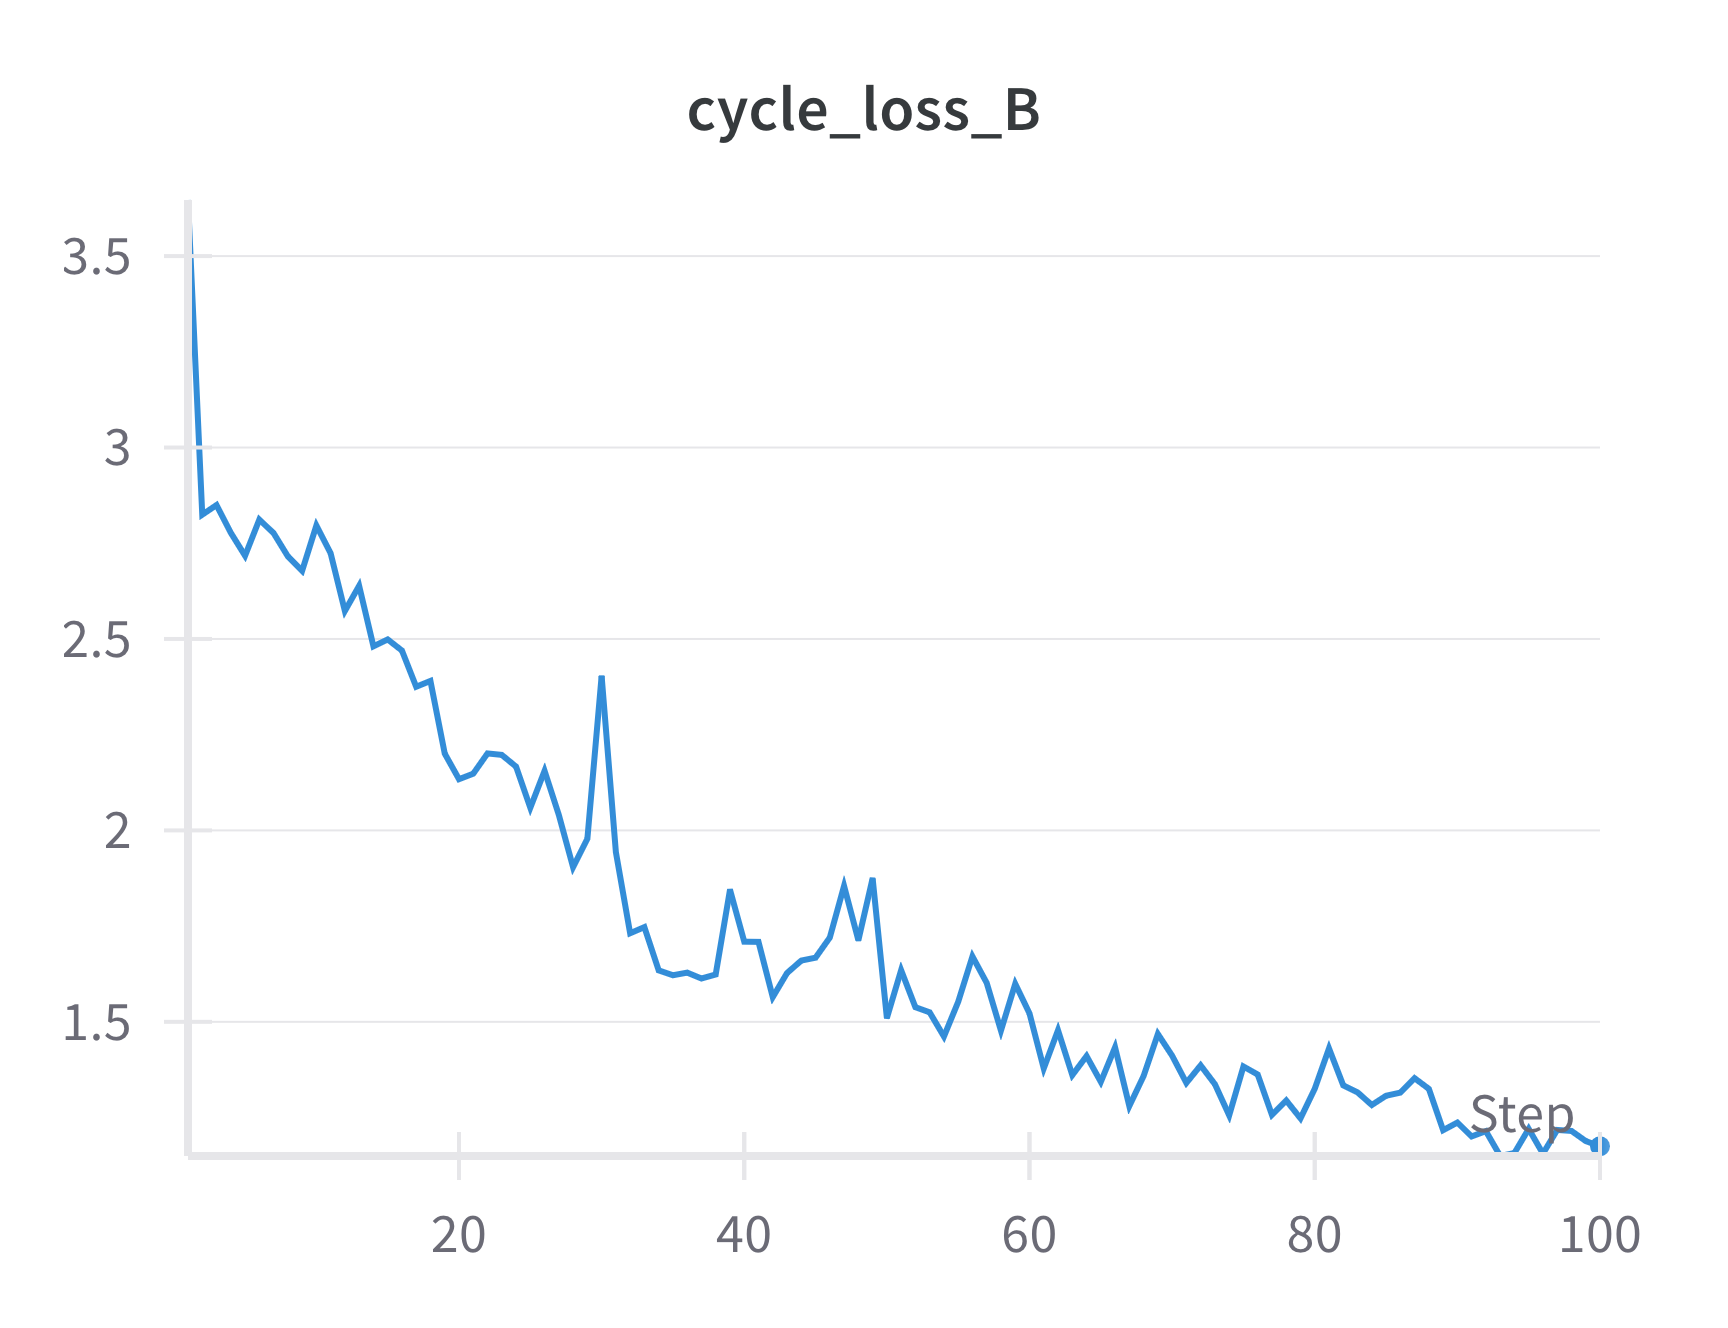
\includegraphics[width=0.45\textwidth]{assets/cycle_loss_B.png}
\caption{Cycle consistency loss for domain B (cycle\_loss\_B)}
\label{fig:cycle_loss_B}
\end{figure}

\begin{figure}[H]
\centering
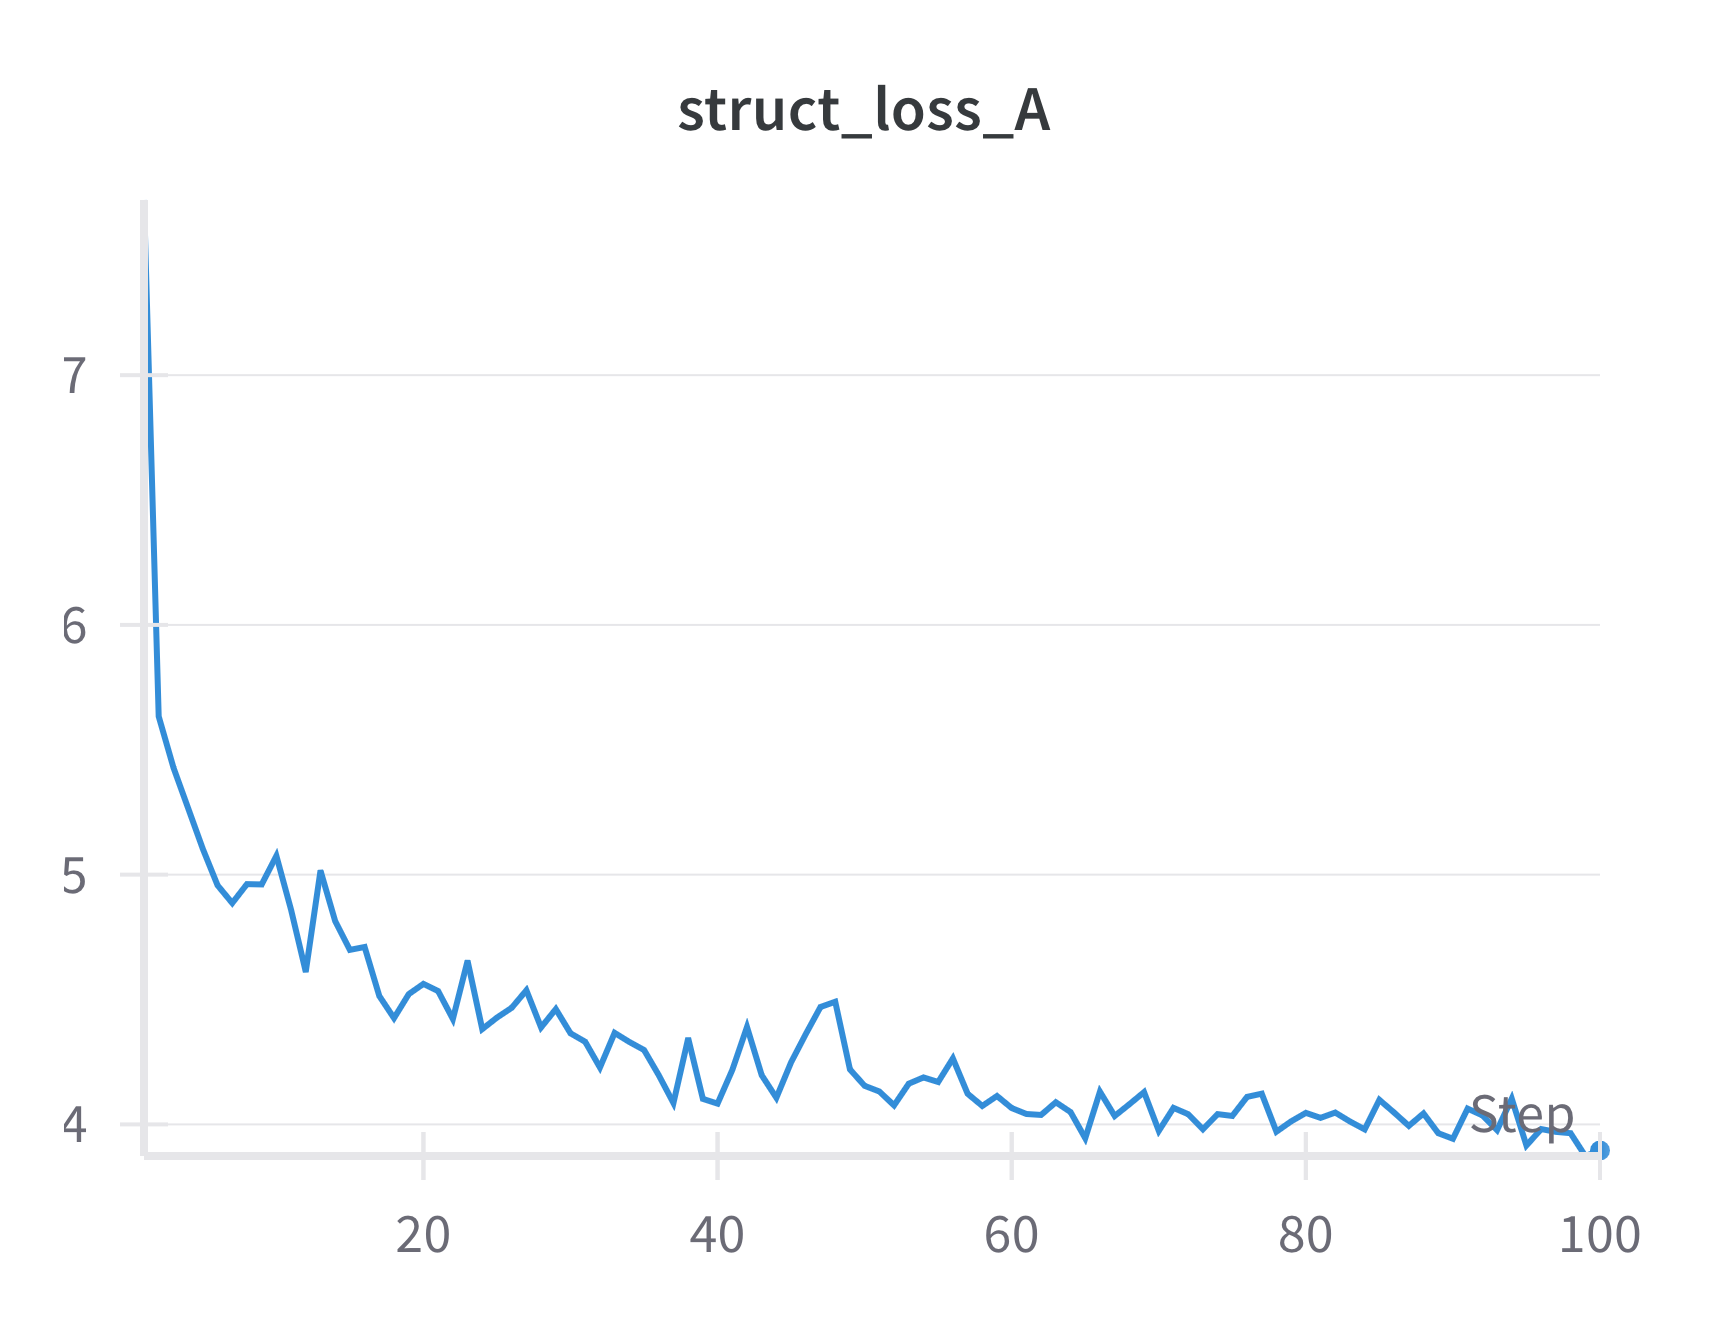
\includegraphics[width=0.45\textwidth]{assets/struct_loss_A.png}
\caption{Structural preservation loss for domain A (struct\_loss\_A)}
\label{fig:struct_loss_A}
\end{figure}

\begin{figure}[H]
\centering
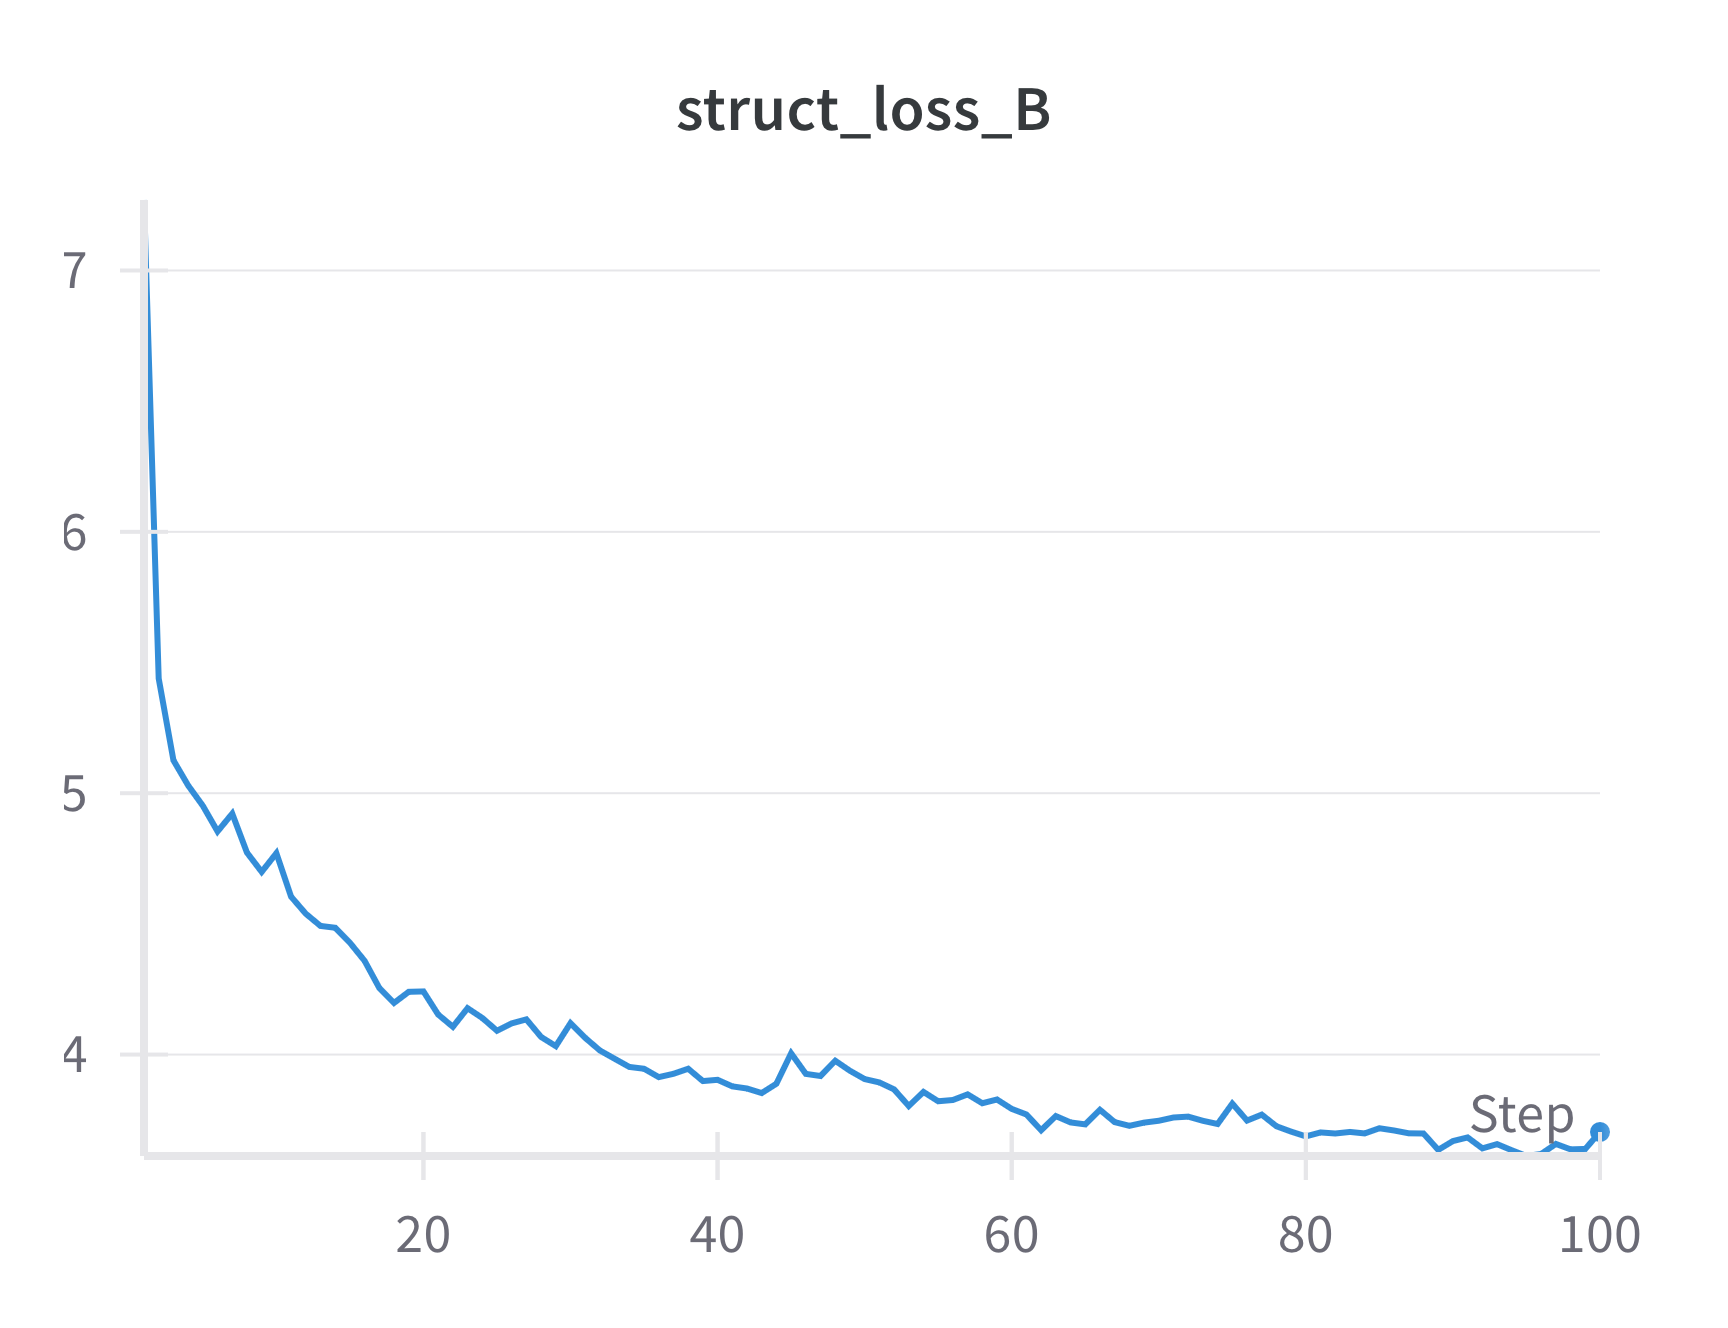
\includegraphics[width=0.45\textwidth]{assets/struct_loss_B.png}
\caption{Structural preservation loss for domain B (struct\_loss\_B)}
\label{fig:struct_loss_B}
\end{figure}

\subsection{Identity Mapping Losses}

\begin{figure}[H]
\centering
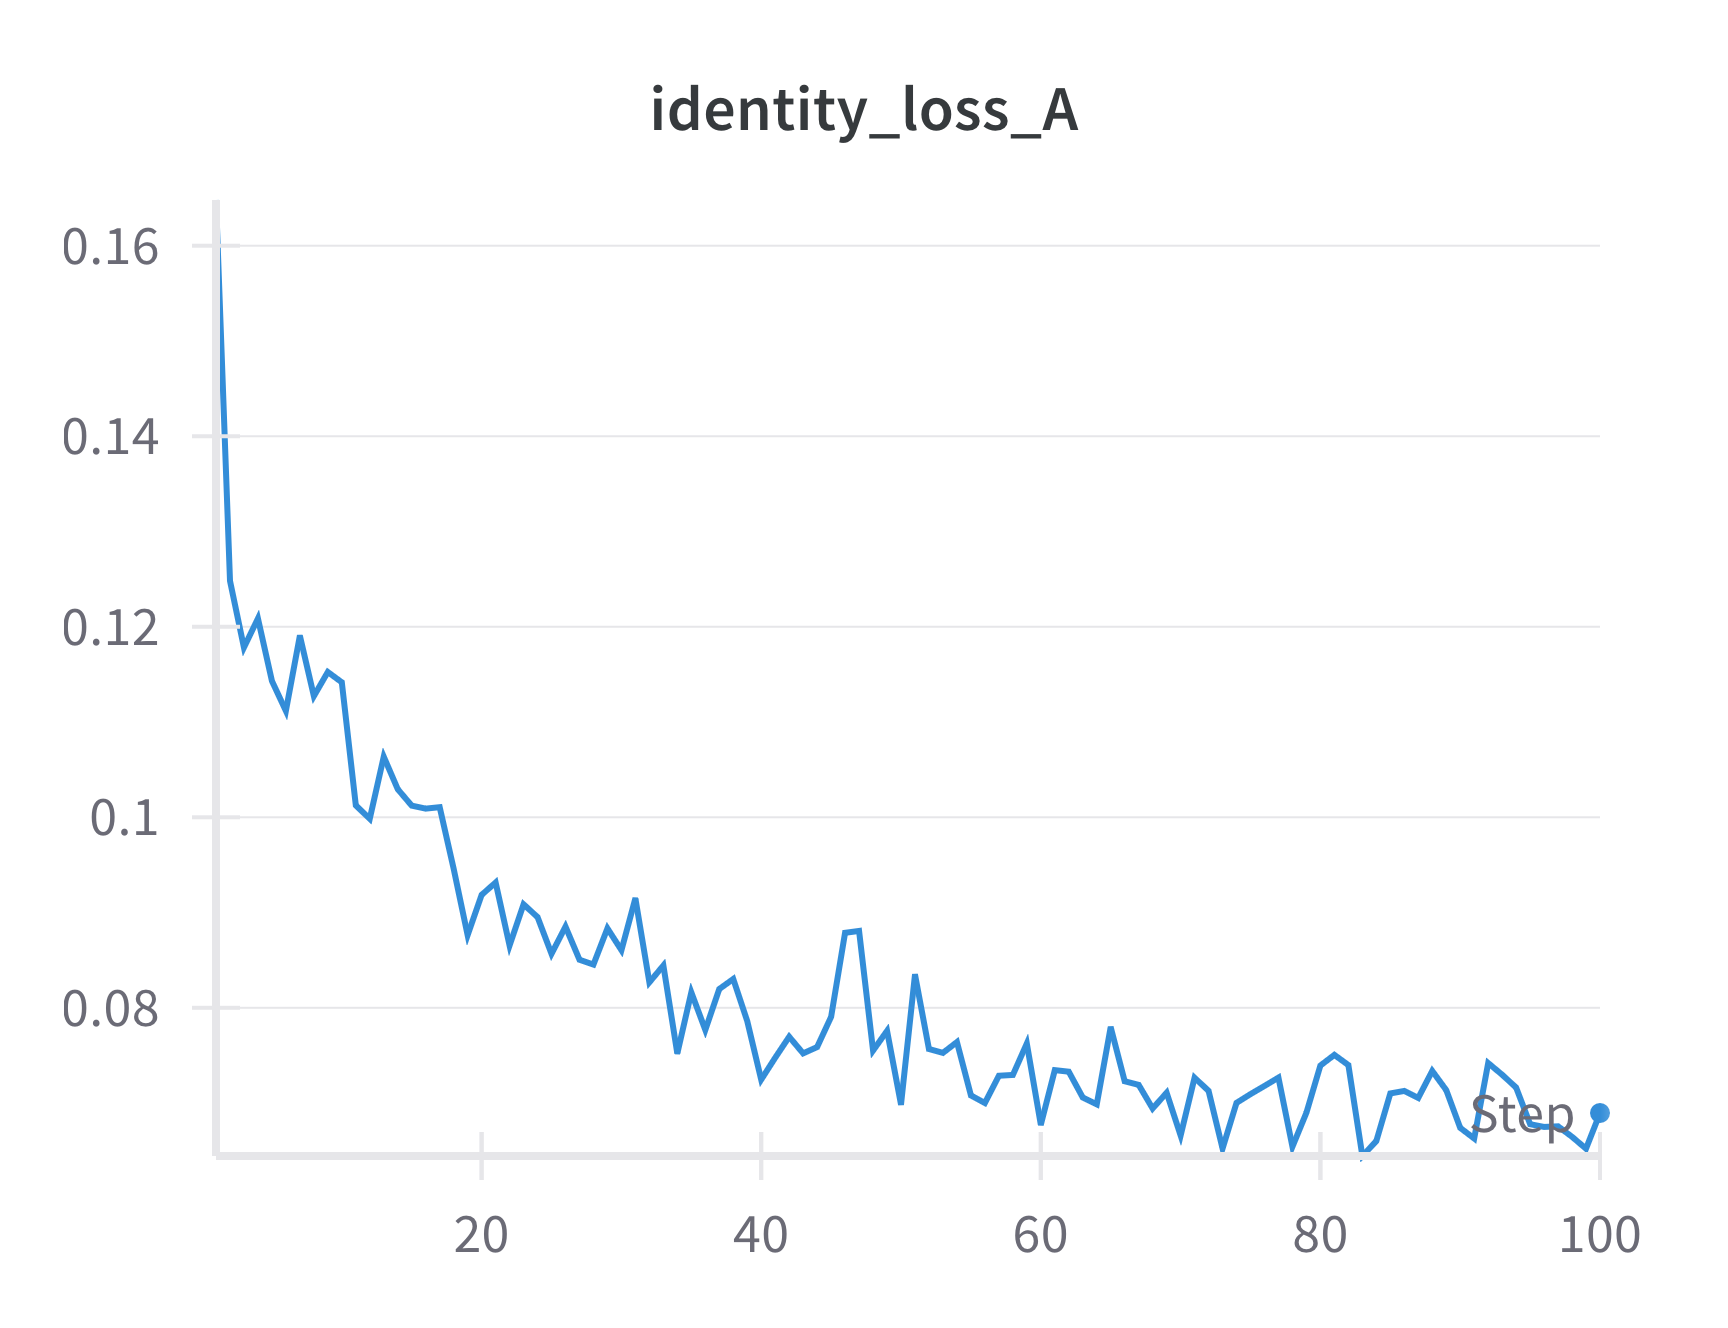
\includegraphics[width=0.45\textwidth]{assets/identity_loss_A.png}
\caption{Identity mapping loss for domain A (identity\_loss\_A)}
\label{fig:identity_loss_A}
\end{figure}

\begin{figure}[H]
\centering
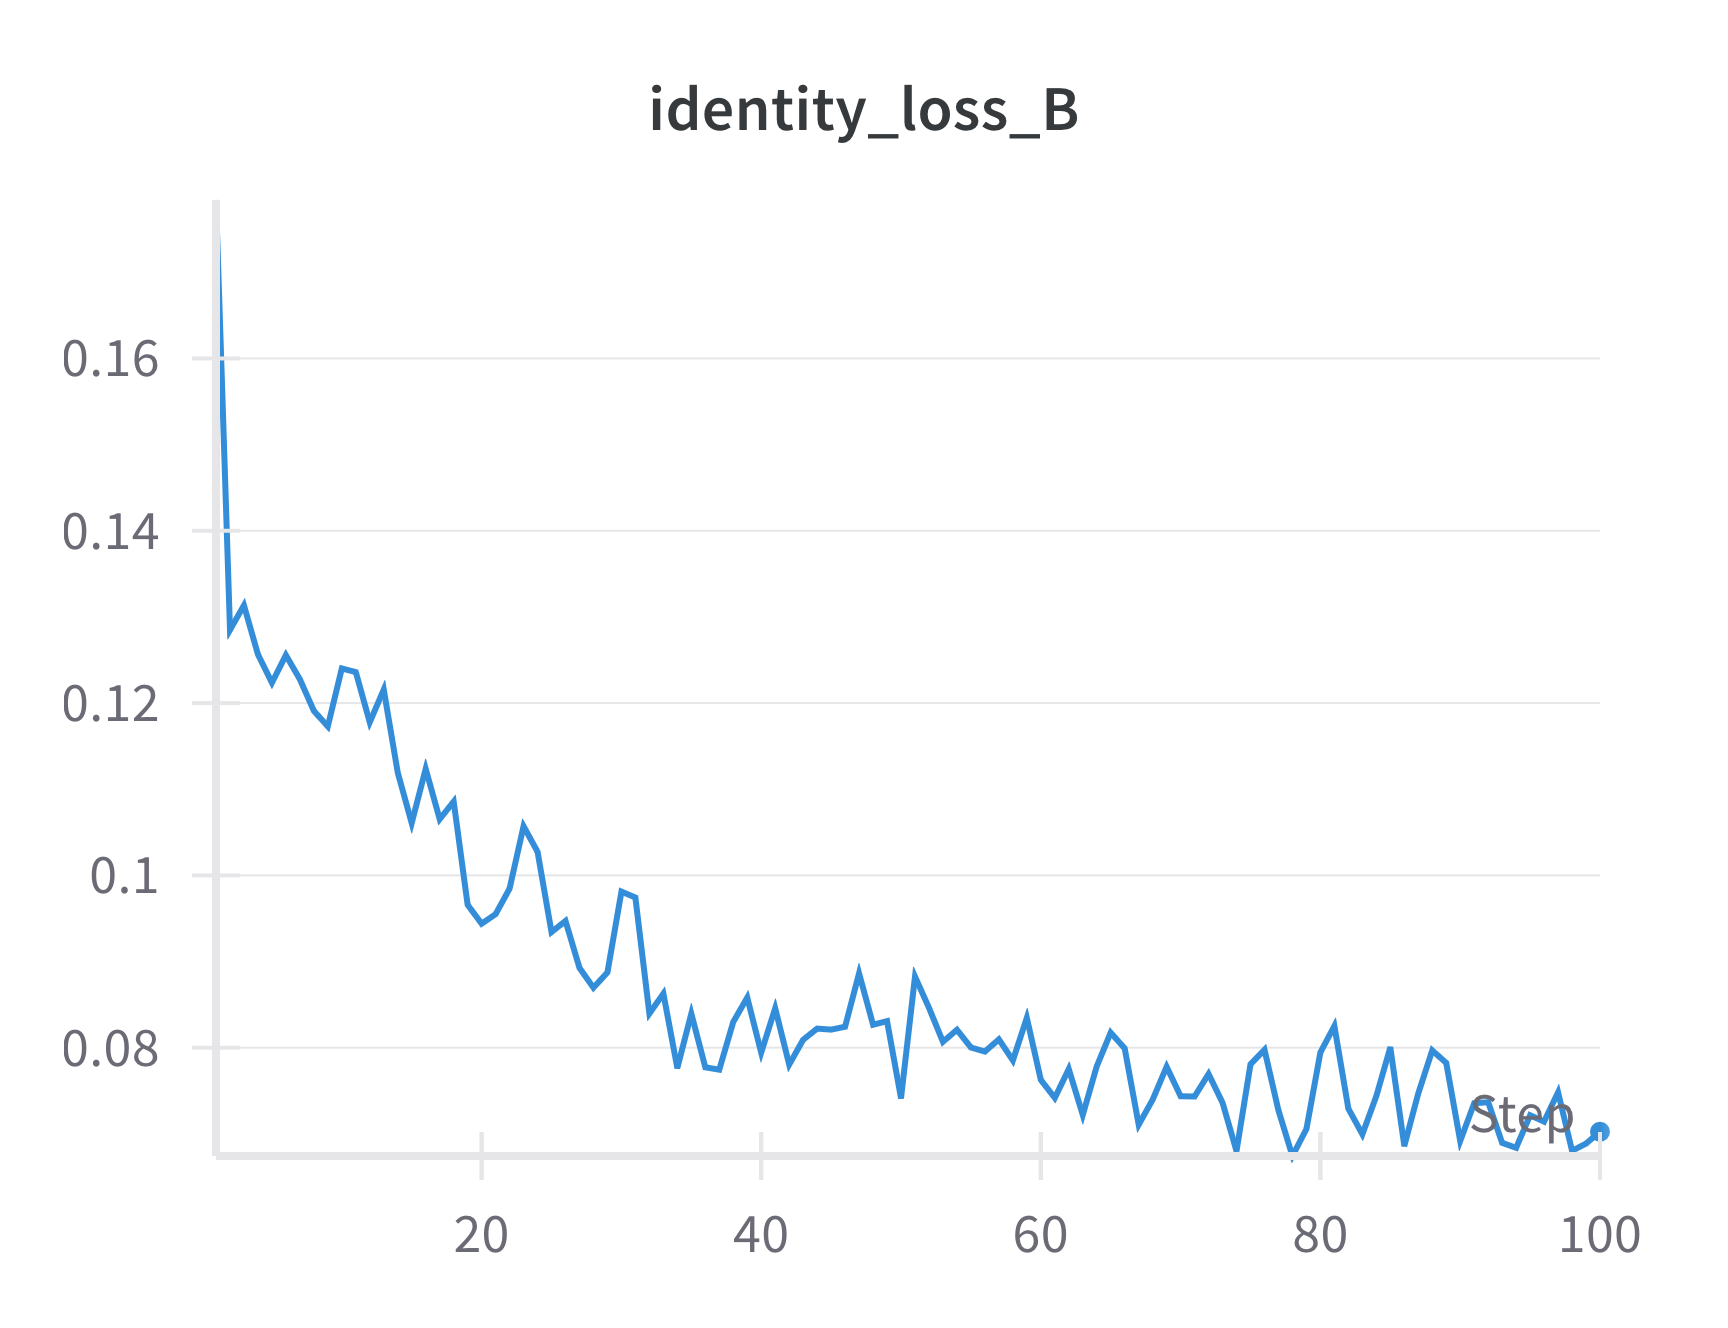
\includegraphics[width=0.45\textwidth]{assets/identity_loss_B.png}
\caption{Identity mapping loss for domain B (identity\_loss\_B)}
\label{fig:identity_loss_B}
\end{figure}

\bibliographystyle{unsrt}
\bibliography{bibliography.bib}

\end{document}